%%%%%%%%%%%%%%%%%%%%%%%%%%%%%%%%%%%%%%%%%%%%%%%%%%%%%%%%%%%%%%%%%%%%%%%%%%%%%%%
% Author:  Pablo Alvarado
%
% Escuela de Ingeniería Electrónica
% Instituto Tecnológico de Costa Rica
%
% Tesis de Licenciatura
% 
% Phone:   +506 2550 9005
% email:   palvarado@itcr.ac.cr
%
%%%%%%%%%%%%%%%%%%%%%%%%%%%%%%%%%%%%%%%%%%%%%%%%%%%%%%%%%%%%%%%%%%%%%%%%%%%%%%%

% \documentclass is book
% If you want a printable two-side version of the thesis
%\documentclass[12pt,twoside,letterpaper]{book}

% If you want an electronic-only version of the thesis, do it one-sided
\documentclass[12pt,oneside,letterpaper]{book}

\usepackage[T1]{fontenc}
%\usepackage[utf8]{inputenc}   % is no longer required (since 2018)
\usepackage{ifthen}            % provide if-then-else operators

% --------------------------------------------------------------------------
% Global variables required in document formatting
% --------------------------------------------------------------------------
%
% BOOK MODE
%
\newboolean{bookmode}                  % boolean used to control book format
% Ensure that only one of the next two lines is active:
\setboolean{bookmode}{true}           % turn book mode on
%\setboolean{bookmode}{false}           % turn book mode off

%
% DRAFT MODE
%   The draft mode activates the TODO index and some "draft" markings all
%   around.  Ensure you set it to false for the final version!!
%   
%
\newboolean{draftmode}                  % boolean used to control draft-mode

%% -------------------------------------------------------------------------

%% Configure su nombre, título de tesis, lectores, fechas, etc. en:
%%
%% >>>>  config.tex  <<<<
%%

% --------------------------------------------------------------------------

% include all packages and define all required general macros
%%%%%%%%%%%%%%%%%%%%%%%%%%%%%%%%%%%%%%%%%%%%%%%%%%%%%%%%%%%%%%%%%%%%%%%%%%%%%%%
% Author:  Pablo Alvarado
%
% Escuela de Electrónica
% Instituto Tecnológico de Costa Rica
%
% Phone:   +506 2550 9005
% email:   palvarado@itcr.ac.cr
% 
%%%%%%%%%%%%%%%%%%%%%%%%%%%%%%%%%%%%%%%%%%%%%%%%%%%%%%%%%%%%%%%%%%%%%%%%%%%%%%%

\PassOptionsToPackage{usenames,dvipsnames}{xcolor}

% -----------------------------------------------------------------------------
%   Define all configuration commands
% -----------------------------------------------------------------------------

\newcommand{\genderLector}[1]{%
  \ifthenelse{\equal{#1}{F}}{%
    Profesora Lectora%
  }{%
    \ifthenelse{\equal{#1}{M}}{%
      Profesor Lector%
    }{%
      Persona profesora lectora%
    }%
  }%
}

% Lector I
\newcommand{\nameLectorI}{$<$\emph{Use defLectorI in config.tex}$>$}
\newcommand{\genderLectorI}{N/A}

\newcommand{\defLectorI}[1][M]{%
  \renewcommand{\genderLectorI}{\genderLector{#1}}%
  \lectorIRelay%
}

\newcommand{\lectorIRelay}[1]{%
  \renewcommand{\nameLectorI}{#1}
}

%% Lector II
\newcommand{\nameLectorII}{$<$\emph{Use setLectorII in main.tex}$>$}
\newcommand{\genderLectorII}{N/A}

\newcommand{\defLectorII}[1][M]{%
  \renewcommand{\genderLectorII}{\genderLector{#1}}%
  \lectorIIRelay%
}

\newcommand{\lectorIIRelay}[1]{%
  \renewcommand{\nameLectorII}{#1}
}

%% Asesor
\newcommand{\nameAsesor}{$<$\emph{Use setAsesor in main.tex}$>$}
\newcommand{\genderAsesor}{$<$\emph{Use setAsesor in main.tex}$>$}

\newcommand{\defAsesor}[1][M]{%
  \ifthenelse{\equal{#1}{F}}{%
    \renewcommand{\genderAsesor}{Profesora Asesora}%
  }{%
    \ifthenelse{\equal{#1}{M}}{%
      \renewcommand{\genderAsesor}{Profesor Asesor}%
    }{%
      % La RAE no ha definido cómo hacer esto...
      %
      % Hay que preguntar a la persona asesora no-binaria directamente
      % cómo gusta ser tratada.
      \renewcommand{\genderAsesor}{Persona profesora asesora}%
    }
  }
  \asesorRelay
}

\newcommand{\asesorRelay}[1]{%
  \renewcommand{\nameAsesor}{#1}
}

% Dates for draft and final
\newcommand{\thesisDraftDate}{\today}
\newcommand{\defDraftDate}[1]{\renewcommand{\thesisDraftDate}{#1}}

\newcommand{\thesisFinalDate}{$<$\emph{Fecha de Defensa en config.tex}$>$}
\newcommand{\defFinalDate}[1]{\renewcommand{\thesisFinalDate}{#1}}

% Author definition and gender related strings

\newcommand{\thesisAuthor}{Error: Undefined}
\newcommand{\thesisAuthorShort}{Error: Undefined}
\newcommand{\thesisAuthorTECID}{Error: Undefined}
\newcommand{\thesisAuthorAddress}{Error: Undefined}
\newcommand{\thesisAuthorDegree}{Error: Undefined}

\newcommand{\defAuthor}[1][M]{%
  \ifthenelse{\equal{#1}{F}}{%
    \renewcommand{\thesisAuthorAddress}{la señora}
    \renewcommand{\thesisAuthorDegree}{Ingeniera}
  }{%
    \ifthenelse{\equal{#1}{f}}{%
      \renewcommand{\thesisAuthorAddress}{la señorita}
      \renewcommand{\thesisAuthorDegree}{Ingeniera}
    }{%
      \ifthenelse{\equal{#1}{M}}{%
        \renewcommand{\thesisAuthorAddress}{el señor}
        \renewcommand{\thesisAuthorDegree}{Ingeniero}
        
      }{%
        \renewcommand{\thesisAuthorAddress}{la persona}
        \renewcommand{\thesisAuthorDegree}{Ingeniere}
      }
    }
  }
  \authorRelay
}

\newcommand{\authorRelay}[1]{%
  \renewcommand{\thesisAuthor}{#1}
}

\newcommand{\defAuthorShort}[1]{%
  \renewcommand{\thesisAuthorShort}{#1}
}

\newcommand{\defAuthorTECID}[1]{%
  \renewcommand{\thesisAuthorTECID}{#1}
}

%% About the institution and department
\newcommand{\thesisDepartment}{Escuela de Ingeniería Electrónica}
\newcommand{\thesisInstitution}{Tecnológico de Costa Rica}

\newcommand{\defDepartment}[1]{%
  \renewcommand{\thesisDepartment}{#1}
}

\newcommand{\defInstitution}[1]{%
  \renewcommand{\thesisInstitution}{#1}
}



%% About the report name, and type
\newcommand{\thesisTitle}{Error: Undefined}
\newcommand{\thesisFlatTitle}{\thesisTitle}
\newcommand{\thesisKeywords}{Error: Undefined}
\newcommand{\thesisType}{Error: Undefined}

%% A tool to remove new lines leaving no spaces
\newcommand\titleFlattener[1]{\def\\{\relax\ifhmode\unskip\fi\space\ignorespaces}#1}

\newcommand{\defTitle}[1]{%
  \renewcommand{\thesisFlatTitle}{\titleFlattener{#1}}
  \renewcommand{\thesisTitle}{#1}
}

\newcommand{\defKeywords}[1]{%
  \renewcommand{\thesisKeywords}{#1}
}

\newcommand{\defTFGType}[1]{%
  \renewcommand{\thesisType}{#1}
}

%% Este archivo contiene toda la configuración básica del documento de
%% tesis, para centralizar alguna información que se requiere en todo
%% el documento.

%% DRAFT MODE

%%   El modo borrador activa las listas de cosas por hacer, con su
%%   índice, y algunas marcas explícitas de "borrador" por todo lado.
%%
%%   Asegúrse de que esta variable sea false en la versión final y de haber
%%   actualizado la fecha de la defensa, un poco más abajo.
\setboolean{draftmode}{true}            % turn draft mode on
%\setboolean{draftmode}{false}          % turn draft mode off

%% Esta es la fecha que se colocará en el modo borrador
\defDraftDate{\today}
%% Esta es la fecha que se usará en la versión final
\defFinalDate{July 16, 2023}

%% Este es el nombre del estudiante y el pronombre que utiliza, para cambiar
%% las portadas como corresponde

% Con el nombre de autor, se debe especificar el género a utilizar:
%
%   [M]asculino
%   [F]emenino (usando "señora" donde corresponda)
%   [f]emenino (usando "señorita" donde corresponda)
%   persona [N]o binaria
%
%   Debido a la falta de norma en español para las personas no binarias,
%   posíblemente deba ajustarse para el gusto de cada quien.
%
\defAuthor[M]{Francis Guindon Badilla}                % Nombre del estudiante
%\defAuthor[f]{María del Pilar Pérez Prado}    % Nombre de la estudiante

\defAuthorShort{F.~Guindon}                      % Nombre corto
\defAuthorTECID{2018259419}                     % Carné

%% Este es el título completo del informe del trabajo final de graduación.
%% Usted puede agregar \\ para forzar líneas nuevas en la portada y automática-
%% mente el comando se encarga de eliminar eso cuando necesita el título
% \defTitle{Detección de artefactos de video \\%
% en tiempo real sobre un sistema embebido}
\defTitle{Embedded soft real time video artifact detector}

%% Palabras clave
\defKeywords{}

%% Tribunal Evaluador
%%
%% Indique los nombres de los lectores y asesor
%% El parámetro opcional es
%%  [M]asculino,
%%  [F]emenino,
%%  persona [N]o binaria
\defAsesor[M]{Dr.\,Pablo Alvarado}
\defLectorI[M]{Dr.\,Jorge Castro Godinez}
\defLectorII[M]{Dr.\,Pablo Mendoza Ponce}


%% Tipo de tesis o informe
%%   - Tesis de Licenciatura
%%   - Informe de Proyecto Final 
%%   - Tesis de Maestría
\defTFGType{Tesis de Licenciatura}

%% Nombre del departamento e institución
\defInstitution{Instituto Tecnológico de Costa Rica}
\defDepartment{Escuela de Ingeniería Electrónica}

 % Load the desired configuration

%Para el PDF (cambiar si se desea otras cosas a lo indicado arriba
\newcommand{\pdfAuthor}{\thesisAuthor}
\newcommand{\pdfTitle}{\thesisFlatTitle} 
\newcommand{\pdfKeywords}{\thesisKeywords}
\newcommand{\pdfSubject}{\thesisType}


%% -------------------------------------------------------------------

\usepackage{ifpdf}

% Command to change between draft or release mode:
\newcommand{\ifdraft}[2]{\ifthenelse{\boolean{draftmode}}{#1}{#2}}
% Command to change between draft or release mode:
\newcommand{\ifbook}[2]{\ifthenelse{\boolean{bookmode}}{#1}{#2}}

% include all required packages here
\usepackage{csquotes}                  % recommended for biblatex
\usepackage[spanish,es-tabla]{babel}   % spanish, remove es-tabla for cuadro
%\usepackage[spanish]{babel}   % spanish, remove es-tabla for cuadro

\usepackage{xspace} % Decide if a space is needed at the end of some commands

\makeatletter
% babel uses a hook and therefore the tablename is here not defined yet.
% However, it defines es@tablename with upper/lowercase, and we use it.
\ifthenelse{\equal{\es@tablename}{Ttabla}}{%
  \newcommand{\cuadro}{tabla}
  \newcommand{\cuadros}{tablas}
  \newcommand{\Cuadro}{Tabla}
  \newcommand{\elcuadro}{la tabla}
  \newcommand{\Elcuadro}{La tabla}
  \newcommand{\loscuadros}{las tablas}
  \newcommand{\Loscuadros}{Las tablas}
  
  \newcommand{\tabla}{tabla}
  \newcommand{\tablas}{tablas}
  \newcommand{\Tabla}{Tabla}
  \newcommand{\latabla}{la tabla}
  \newcommand{\Latabla}{La tabla}
  \newcommand{\lastablas}{las tablas}
  \newcommand{\Lastablas}{Las tablas}
  
  \newcommand{\tabref}[1]{\hyperref[#1]{tabla~\ref*{#1}}\xspace}
  \newcommand{\Tabref}[1]{\hyperref[#1]{Tabla~\ref*{#1}}\xspace}

  \newcommand{\latabref}[1]{la \tabref{#1}}
  \newcommand{\Latabref}[1]{La \tabref{#1}}

}{%
  \newcommand{\cuadro}{cuadro}
  \newcommand{\cuadros}{cuadros}
  \newcommand{\Cuadro}{Cuadro}
  \newcommand{\elcuadro}{el cuadro}
  \newcommand{\Elcuadro}{El cuadro}
  \newcommand{\loscuadros}{los cuadros}
  \newcommand{\Loscuadros}{Los cuadros}
  
  \newcommand{\tabla}{cuadro}
  \newcommand{\tablas}{cuadros}
  \newcommand{\Tabla}{Cuadro}
  \newcommand{\latabla}{el cuadro}
  \newcommand{\Latabla}{El cuadro}
  \newcommand{\lastablas}{los cuadros}
  \newcommand{\Lastablas}{Los cuadros}
  
  \newcommand{\tabref}[1]{\hyperref[#1]{cuadro~\ref*{#1}}\xspace}
  \newcommand{\Tabref}[1]{\hyperref[#1]{Cuadro~\ref*{#1}}\xspace}

  \newcommand{\latabref}[1]{el \tabref{#1}}
  \newcommand{\Latabref}[1]{El \tabref{#1}}

}
\makeatother

% References to figures
\newcommand{\figref}[1]{\hyperref[#1]{figura~\ref*{#1}}\xspace}
\newcommand{\Figref}[1]{\hyperref[#1]{Figura~\ref*{#1}}\xspace}
\newcommand{\lafigref}[1]{la \hyperref[#1]{figura~\ref*{#1}}\xspace}
\newcommand{\Lafigref}[1]{La \hyperref[#1]{figura~\ref*{#1}}\xspace}

% References to equations
\newcommand{\equ}[1]{\hyperref[#1]{(\ref*{#1})}\xspace}

% Refrences to chapters and sections
\newcommand{\capref}[1]{\hyperref[#1]{capítulo~\ref{#1}}\xspace}
\newcommand{\secref}[1]{\hyperref[#1]{sección~\ref{#1}}\xspace}

\usepackage{makeidx}                    % to create index file

\usepackage[nottoc]{tocbibind}          % Fix the hyperrefs to TOC,TOF, etc.
                                        % and ensure that they appear all in 
                                        % the Table of Contents
\ifdraft{%
  %\usepackage[refpage]{nomencl}        % Use to easily administrate the list
  \usepackage[intoc,spanish]{nomencl}   % of symbols
}{%
  \usepackage[intoc,spanish]{nomencl}
}

\usepackage{siunitx}                    % Units of the SI
\sisetup{output-decimal-marker = {,}}   % Use decimal , instead of decimal .
\DeclareSIQualifier\peak{p}
\DeclareSIQualifier\ppeak{pp}

\usepackage{amsmath}
\usepackage{amssymb,amstext}            % AMS-math and symbols package
\usepackage{mathrsfs}                   % Calygraphic fonts for transforms
\usepackage{trsym}                      % Para símbolos de transformadas o---o
\usepackage{stmaryrd}                   % For short arrows
\usepackage{nicefrac}
\usepackage{array}                      % extensions to tabular environment
\usepackage{longtable}                  % supports extraordinary long tables
\usepackage{tabularx}                   % supports tables with fixed width

\usepackage[backend=biber,              % Use biber/biblatex
            style=ieee,
            sorting=none,
            citestyle=numeric-comp]{biblatex}

\usepackage{afterpage}                  % put something only after the page
\usepackage{multirow}                   % supports multiple row grouping in 
                                        % tables
\usepackage{multicol}                   % multiple columns environments
\usepackage{enumitem}                   % better enumeration with paralist 
                                        % equivalents as follows:

\newlist{compactitem}{itemize}{3}
\setlist[compactitem]{topsep=0pt,partopsep=0pt,itemsep=0pt,parsep=0pt}
\setlist[compactitem,1]{label=\textbullet}
\setlist[compactitem,2]{label=---}
\setlist[compactitem,3]{label=*}

\newlist{compactdesc}{description}{3}
\setlist[compactdesc]{topsep=0pt,partopsep=0pt,itemsep=0pt,parsep=0pt}

\newlist{compactenum}{enumerate}{3}
\setlist[compactenum]{label*=\arabic*.,topsep=0pt,partopsep=0pt,itemsep=0pt,parsep=0pt}
\newlist{compactenuma}{enumerate}{3}
\setlist[compactenuma]{label*=\alph*.,topsep=0pt,partopsep=0pt,itemsep=0pt,parsep=0pt}

\usepackage{icomma}                     % decimal comma in math mode

\usepackage{bold-extra}

\usepackage[format=hang,%
            font=small,%
            labelfont=bf]{caption}      % nicer figure captions
\usepackage{subcaption}                 % for subfigures
            
\usepackage{booktabs}                   % book type tabulars
\usepackage{pdfpages}                   % used to include the final "acta"

% the own style with options depending on the draft mode
\ifdraft{%
\usepackage[todo]{sty/tecStyle}         % some command definitions
                                        % options [todo] todo-index
}{%
\usepackage{sty/tecStyle}               % some command definitions
                                        % options [todo] todo-index
}

%% fix the title for examples
\renewcommand{\examplelistname}{Índice de ejemplos}
\renewcommand{\examplename}{Ejemplo}

%% define some command to cope with the tribunal names

%% Lector I


\usepackage{url}                        % allows linebreaks at certain
                                        % characters or combinations of 
                                        % characters for URLs

%% Usual tikz libraries and configuration
\usepackage{tikz}
\usepackage{pgfplots}
\pgfplotsset{compat=1.16}
\usepgfplotslibrary{fillbetween}
\usetikzlibrary{patterns,shapes,arrows.meta,positioning,calc,babel}
\usetikzlibrary{fit,shapes.geometric,decorations.markings}

\usepackage{listings}                   % syntax highlighting of code fragments

\lstdefinestyle{verilog-style}
{
  language=Verilog,
  basicstyle=\small\ttfamily,
  keywordstyle=\color{dkblue},
  identifierstyle=\color{black},
  commentstyle=\color{dkgreen},
  numbers=left,
  numberstyle=\tiny\color{black},
  numbersep=10pt,
  tabsize=8,
  moredelim=*[s][\colorIndex]{[}{]},
  literate=*{:}{:}1
}
\lstset{literate=%
  {á}{{\'a}}1
  {é}{{\'e}}1
  {í}{{\'i}}1
  {ó}{{\'o}}1
  {ú}{{\'u}}1
  {ñ}{{\~n}}1
  {Á}{{\'A}}1
  {É}{{\'E}}1
  {Í}{{\'I}}1
  {Ó}{{\'O}}1
  {Ú}{{\'U}}1
  {Ñ}{{\~N}}1
}

\definecolor{vorange}{RGB}{255,143,102}

\makeatletter
\newcommand*\@lbracket{[}
\newcommand*\@rbracket{]}
\newcommand*\@colon{:}
\newcommand*\colorIndex{%
    \edef\@temp{\the\lst@token}%
    \ifx\@temp\@lbracket \color{black}%
    \else\ifx\@temp\@rbracket \color{black}%
    \else\ifx\@temp\@colon \color{black}%
    \else \color{vorange}%
    \fi\fi\fi
}
\makeatother


% For pdflatex
% - The hyperref package should always be loaded last, since it has to
%   overwrite some of the commands.
% - The package subfigure caused that the pagebackrefs and index refs were set
%   incorrectly.

\ifpdf
%
% final / draft document options
%\usepackage{graphicx}                   % for inserting pdf-graphics.
                                        % options final / draft
\ifdraft{%
\usepackage[%pdftex,%
            naturalnames=true,
            linktocpage,
            hyperindex,
            colorlinks,
            urlcolor=dkred,          %\href to external url
            filecolor=dkmagenta,     %\href to local file
            linkcolor=dkred,         %\ref and \pageref
            citecolor=dkgreen,       %\cite
            plainpages=false,
            pdfpagelabels,
            pdfpagemode=UseOutlines, % means use bookmarks (None,UseOutlines)
            % bookmarksopen=false,   % would show the whole hierarchy if true
            bookmarksnumbered=true,
            pdfpagelayout=OneColumn, % SinglePage,OneColumn,TwoColumnLeft,...
            pdfview=FitH, % FitB,FitBH,FitBV,Fit,FitH,FitV
            pdfstartview=FitH, % FitB,FitBH,FitBV,Fit,FitH,FitV
            unicode,
            ]{hyperref}
}{%
% Use biber/biblatex
\usepackage[%pdftex,%
            naturalnames=true,
            linktocpage,hyperindex,
            colorlinks,
            urlcolor=dkred,          %\href to external url
            filecolor=dkmagenta,     %\href to local file
            linkcolor=dkred,         %\ref and \pageref
            citecolor=dkgreen,       %\cite
            plainpages=false,
            pdfpagelabels,
            pdfpagemode=UseOutlines, % means use bookmarks (None,UseOutlines)
            % bookmarksopen=false,   % open the whole hierarchy if true!
            bookmarksnumbered=true,
            pdfpagelayout=OneColumn, % SinglePage,OneColumn,TwoColumnLeft,...
            pdfview=FitH, % FitB,FitBH,FitBV,Fit,FitH,FitV
            pdfstartview=FitH, % FitB,FitBH,FitBV,Fit,FitH,FitV,
            unicode,
            ]{hyperref}
}


%
% Ensure that the links of the images point to the top of the images and not
% to the caption
%
\usepackage[figure]{hypcap}

% %
% % Ensure that pdfLaTeX do the same spacing as LaTeX
% %
\pdfadjustspacing=1 
% %
\else   % i.e. if not pdf

\usepackage[active]{srcltx}             % insert links into the dvi to jump
\usepackage{graphicx}                   % for inserting eps-graphics.
                                        % options final / draft
                                        % into the sources directly.
\ifdraft{%
\usepackage[ps2pdf,%
            % plainpages=false,
            linktocpage,
            hyperindex,
            % pdfpagelabels,
            pdfpagemode=UseOutlines,
            pdfstartview=FitH,
            unicode,]{hyperref}
}{%
\usepackage[ps2pdf,%
            % plainpages=false,
            linktocpage,
            hyperindex,
            % pdfpagelabels,
            pdfpagemode=UseOutlines,
            pdfstartview=FitH,
            unicode,]{hyperref}
}

%\usepackage[ps2pdf]{hyperref}

\fi  % end of if pdf or not

% --------------------------------------------------------------------------

% Allow the use of international characters
\AtBeginDocument{%
  \hypersetup{%
             pdftitle={\pdfTitle},%
             pdfsubject={\pdfSubject},%
             pdfauthor={\pdfAuthor},%
             pdfkeywords={\pdfKeywords}
            }%
}


%\usepackage{algorithmic}            % algorithmic environment


\usepackage{rotating}                % allow block rotation

%% This environment will allow to rotate a page in the PDF, just
%% for visualization purposes.  Since nowadays the documents are
%% almost never printed, it is best if rotated pages are also shown
%% rotated in the PDF viewer, and this is the purpose of this environment.
\newenvironment{rotatepage}%
{\global\pdfpageattr\expandafter{\the\pdfpageattr/Rotate 90}}%
{\clearpage\pagebreak[4]\global\pdfpageattr\expandafter{\the\pdfpageattr/Rotate 0}}

    
%%%%%%%%%%%%%%%%%%%%%%%%%%%%%%%%%%%%%%%%%%%%%%%%%%%%%%%%%%%%%%%%%%%%%%%%%%%%%%%

%\sloppy

%
% Some own font definitions
%
\DeclareMathAlphabet{\mathpzc}{OT1}{pzc}{m}{it}
\DeclareMathAlphabet{\mathpss}{OT1}{cmss}{m}{sl}

%
% page layout
%

\usepackage{vmargin}
\setpapersize{USletter}

% For letter-paper printing
\setmarginsrb{33mm}{8mm}{23mm}{7mm}{15pt}{15pt}{7mm}{12mm}
%\setlength{\headheight}{15pt}         % fancy headers wanted this

%
% Fraction of Float Object / Text
%

\renewcommand{\topfraction}{0.95}       % how much of top of page should be 
                                        % allowed to be float object?
\renewcommand{\bottomfraction}{0.95}    % how much of bottom of page should be
                                        % allowed to be float object?
\renewcommand{\textfraction}{0.05}      % how much of page must be text?

\usepackage{fancyhdr}                   % fancy page headers

\usepackage{lastpage}

%
% header and footer layout (needs package fancyhdr)
%
\newcommand{\copyrightfooter}{\tiny{\copyright \the\year\ --- \thesisAuthorShort %
    \qquad Uso exclusivo ITCR}}
%
\newcommand{\draftfoot}%
  {\ifdraft{\textcolor{dkblue}{\tiny\textsl{Borrador: \today}}{}}
           {}
}

\pagestyle{fancy}
\renewcommand{\chaptermark}[1]{\markboth{{\small
    \thechapter\hspace*{1mm}#1}}{}}
\renewcommand{\sectionmark}[1]{\markright{{\small
    \thesection\hspace*{1mm}#1}}{}}
%\lhead[{\small\textsc\Roman{\thepage}}]{\fancyplain{}%
\lhead[{\small\thepage}]{\fancyplain{}%
        {{\slshape \small\nouppercase{\leftmark}}}}
\chead[]{}
\rhead[\fancyplain{}%
%        {{\slshape \small\nouppercase{\rightmark}}}]{{\small\textsc\Roman{\thepage}}}
        {{\slshape \small\nouppercase{\rightmark}}}]{{\small\thepage}}
\lfoot[]{\draftfoot}
\ifbook{%
  \cfoot[]{}
}{
  \cfoot[\copyrightfooter]{\copyrightfooter}
}
\rfoot[\draftfoot]{}
\renewcommand{\headrulewidth}{0.5pt}
\renewcommand{\footrulewidth}{0pt}

%
% Caption style for tables
% For caption v3:
\captionsetup[table]{position=top,
  format=hang,
  textfont={normalsize},
  labelfont={normalsize,bf}}

\newcommand{\tablecaption}[2][foo]{%
  \ifthenelse{\equal{#1}{foo}}{%
    \caption{#2}%
  }{%
    \caption[#1]{#2}%
  }
}

%% En español hay diferencia entre Tabla y Cuadro.
%%
%% Tabla: es la tabla periódica, o una tabla de logaritmos o de
%%        probabilidades o de integrales. Usualmente es algo que no
%%        requiere referencias o explicaciones adicionales en el texto porque
%%        todas sus entradas son sucesiones de alguna cosa que se busca allí
%%        mismo
%% Cuadro: es lo que usualmente se usa en inglés como "table", y resume
%%        información que requiere al menos parcialmente explicaciones en el
%%        el texto.

%% \addto\extrasspanish{\renewcommand{\tablename}{Tabla}}
%% \addto\extrasspanish{\renewcommand{\listtablename}{\'Indice de tablas}}

%
% paragraph layout
%
\renewcommand{\baselinestretch}{1.1}    % line spacing
\parindent0em                           % indentation width of first line
\parskip1.3ex                           % space between paragraphs

%
% document consists of
% chapter - section - subsection - subsubsection - paragraph - subparagraph
%
\setcounter{secnumdepth}{2}             % depth of section numbering
\setcounter{tocdepth}{2}                % depth of table of contents

% For biblatex
\addbibresource{literatura.bib}

%
% prepares index from entries like \index{word} or \index{group!word}.
% don't forget to call "makeindex filename" for final index generation.
%
\makeindex                            %% for package makeidx.sty
%\newindex{default}{idx}{ind}{Index}  %% for package index.sty

\newcommand{\octave}{GNU/Octave}
\newcommand{\linux}{GNU/Linux}


%
% prepares notation or nomenclature 
%
\makenomenclature

%%% Local Variables: 
%%% mode: latex
%%% TeX-master: "main"
%%% End: 


% define all symbols used in the document
%% ---------------------------------------------------------------------------
%% paNotation.tex
%%
%% Notation
%%
%% $Id: notation.tex 1467 2010-07-24 16:47:17Z palvarado $
%% ---------------------------------------------------------------------------

\newcommand{\nms}{\negmedspace}

%%
% Command definitions for localized symbol format definition
%%
\renewcommand{\Re}{\operatorname{Re}}
\renewcommand{\Im}{\operatorname{Im}}

\newcommand{\prt}[1]{\ensuremath{\mathcal{#1}}}         %% partitioning
\newcommand{\img}[1]{\ensuremath{\mathcal{#1}}}         %% image as a set
\newcommand{\reg}[1][R]{\ensuremath{\mathcal{#1}}}      %% region
\newcommand{\pred}[1]{\ensuremath{\mathrm{#1}}}         %% predicate
\newcommand{\operat}[2]{\mathcal{#1}\left\{#2\right\}}
\newcommand{\transf}[1]{\mathscr{#1}}
\newcommand{\fourier}[1]{\transf{F}\left\{#1\right\}}
\newcommand{\ifourier}[1]{\transf{F}^{-1}\left\{#1\right\}}
\newcommand{\laplace}[1]{\transf{L}\left\{#1\right\}}
\newcommand{\ulaplace}[1]{\transf{L}_u\left\{#1\right\}}
\newcommand{\blaplace}[1]{\transf{L}_b\left\{#1\right\}}
\newcommand{\ilaplace}[1]{\transf{L}^{-1}\left\{#1\right\}}
\newcommand{\ztrans}[1]{\transf{Z}\left\{#1\right\}}
\newcommand{\iztrans}[1]{\transf{Z}^{-1}\left\{#1\right\}}
\newcommand{\zutrans}[1]{\transf{Z}_u\left\{#1\right\}}
\newcommand{\exceq}{\ensuremath{\overset{!}{=}}}

\newcommand{\signum}{\operatorname{signum}}
\newcommand{\vct}[1]{\ensuremath{\underline{\mathbf{#1}}}}
\newcommand{\mat}[1]{\ensuremath{\mathbf{#1}}}
\newcommand{\vctmu}{\vct{\boldsymbol{\mu}}}
\newcommand{\vctzeta}{\vct{\boldsymbol{\zeta}}}
\newcommand{\vctpi}{\vct{\boldsymbol{\pi}}}
\newcommand{\vctvarphi}{\vct{\boldsymbol{\varphi}}}
\newcommand{\raum}[1]{\ensuremath{\mathbb{#1}}}
\newcommand{\matSigma}{\mat{\boldsymbol{\Sigma}}}
\newcommand{\matLambda}{\mat{\boldsymbol{\Lambda}}}
\newcommand{\matPsi}{\mat{\boldsymbol{\Psi}}}
\newcommand{\matPhi}{\mat{\boldsymbol{\Phi}}}
\newcommand{\row}[2]{\ensuremath{\mathbf{\underline{#1}_{#2(\cdot)}}}}
\newcommand{\col}[2]{\ensuremath{\mathbf{\underline{#1}_{(\cdot) #2}}}}
\newcommand{\seq}[1]{\ensuremath{#1}}
\newcommand{\set}[1]{\ensuremath{\mathcal{#1}}}
\newcommand{\gset}[1]{\ensuremath{#1}} %% set for greek symbols
\newcommand{\front}[1]{\widehat{\set{#1}}}
\newcommand{\setlambda}{\set{\boldsymbol{\lambda}}}
\newcommand{\klass}[1]{\ensuremath{\mathpss{#1}}}
\newcommand{\graph}[1]{\ensuremath{\mathsf{#1}}}
\newcommand{\lab}[1]{\ensuremath{\mathpss{L}(#1)}}
\newcommand{\myfrac}[2]{{\footnotesize #1/#2}}
\newcommand{\ifthenspc}{\rule{3mm}{0mm}}
\newcommand{\point}[1]{\ensuremath{\mathsf{#1}}}
\newcommand{\estim}[1]{\ensuremath{\hat{#1}}}
\newcommand{\numset}[1]{\ensuremath{\mathbb{#1}}}
\newcommand{\tuple}[1]{\ensuremath{\left\langle#1\right\rangle}}
\newcommand{\norm}[1]{\ensuremath{\left\lVert#1\right\rVert}}
\newcommand{\conj}[1]{\ensuremath{{{#1}^{\ast}}}}
\newcommand{\base}[1]{\set{#1}}
\newcommand{\zeron}[1]{\ensuremath{\underset{\uparrow}{#1}}}
\newcommand{\sysT}{\ensuremath{\mathcal{T}}}
\newcommand{\sys}[1]{\ensuremath{\sysT\left[#1\right]}}
%\newcommand{\sen}{\operatorname{sen}} % sinus in spanish (seno)
%\newcommand{\senh}{\operatorname{senh}} % sinus hiperbolicus in spanish (seno)
%\newcommand{\arcsen}{\operatorname{arcsen}} % arcus sinus hiperbolicus in spanish (arcoseno)
\newcommand{\sgn}{\operatorname{sgn}} % signus
\newcommand{\roc}{\text{ROC: }}

\newcommand{\code}[1]{\texttt{#1}}
\newcommand{\conv}{\ensuremath{\ast}}
\newcommand{\cconv}{\ensuremath{\;\,\text{\footnotesize{N}}\!\!\!\!\!\!\bigcirc}}
\newcommand{\Ln}{\operatorname{Ln}}
\newcommand{\rand}{\operatorname{rand}}
\newcommand{\sa}{\operatorname{sa}}
\newcommand{\senc}{\operatorname{senc}}


%% Natural, Integer and Real Numbers
\newcommand{\setA}{\ensuremath{\mathbb{A}}}
\newcommand{\setB}{\ensuremath{\mathrm{I\negthinspace B}}}
\newcommand{\setC}{\ensuremath{\mathbb{C}}}
\newcommand{\setD}{\ensuremath{\mathrm{I\negthinspace D}}}
\newcommand{\setE}{\ensuremath{\mathrm{I\negthinspace E}}}
\newcommand{\setF}{\ensuremath{\mathrm{I\negthinspace F}}}
\newcommand{\setG}{\ensuremath{\mathbb{G}}}
\newcommand{\setH}{\ensuremath{\mathrm{I\negthinspace H}}}
\newcommand{\setI}{\ensuremath{\mathbb{I}}}
\newcommand{\setJ}{\ensuremath{\mathbb{J}}}
\newcommand{\setK}{\ensuremath{\mathrm{I\negthinspace K}}}
\newcommand{\setL}{\ensuremath{\mathrm{I\negthinspace L}}}
\newcommand{\setM}{\ensuremath{\mathrm{I\negthinspace M}}}
\newcommand{\setN}{\ensuremath{\mathrm{I\negthinspace N}}}
\newcommand{\setO}{\ensuremath{\mathbb{O}}}
\newcommand{\setP}{\ensuremath{\mathrm{I\negthinspace P}}}
\newcommand{\setQ}{\ensuremath{\mathbb{Q}}}
\newcommand{\setR}{\ensuremath{\mathrm{I\negthinspace R}}}
\newcommand{\setS}{\ensuremath{\mathbb{S}}}
\newcommand{\setT}{\ensuremath{\mathbb{T}}}
\newcommand{\setU}{\ensuremath{\mathbb{U}}}
\newcommand{\setV}{\ensuremath{\mathbb{V}}}
\newcommand{\setW}{\ensuremath{\mathbb{W}}}
\newcommand{\setX}{\ensuremath{\mathbb{X}}}
\newcommand{\setY}{\ensuremath{\mathbb{Y}}}
\newcommand{\setZ}{\ensuremath{\mathbb{Z}}}


%%
% Multimap symbols
%
\newcommand{\ttoF}{\,\circ\!\negthickspace\longrightarrow\negthickspace\!\negthickspace\bullet\,}
\newcommand{\Ftot}{\,\bullet\negthickspace\!\negthickspace\longleftarrow\!\negthickspace\circ\,}
\newcommand{\ttoZ}{\ttoF}
\newcommand{\Ztot}{\Ftot}
\newcommand{\ttoZu}{\overset{z_u}{\ttoF}}
\newcommand{\Zutot}{\overset{z_u}{\Ftot}}
\newcommand{\vttoF}{\text{\begin{sideways}$\Ftot$\end{sideways}}}
\newcommand{\vFtot}{\text{\begin{sideways}$\ttoF$\end{sideways}}}
\newcommand{\vttoZ}{\vttoF}
\newcommand{\vZtot}{\vFtot}
\newcommand{\ttoDF}{\underset{N}{\ttoF}}
\newcommand{\DFtot}{\underset{N}{\Ftot}}

\newcommand{\thisis}[2]{\underset{#1}{\underbrace{#2}}}

%%% Local Variables:
%%% mode: latex
%%% TeX-master: "paMain"
%%% End:


% allow equations to be splitted (breaked) into several pages
\allowdisplaybreaks[3]

% Added by francis
%\usepackage{import}


% --------------------------------------------------------------------------
\begin{document}
  % where to look for graphics
  \graphicspath{{./}{./fig/}}

  \pagenumbering{alph}
  % fix some terms not activated due to the bug of hyperref with spanish.
  
  \renewcommand{\examplesolution}{Solución}
  \pagestyle{empty}

  % select one of the following titlepages
  %%% ---------------------------------------------------------------------------
%% titlepage_licce_es.tex
%%
%% Title page
%%
%% $Id: titlepage.tex 1452 2010-07-07 00:55:16Z palvarado $
%% ---------------------------------------------------------------------------
\phantomsection
\pdfbookmark[1]{Portada}{Portada}

\thispagestyle{empty} 

\begin{center}

Tecnológico de Costa Rica

\par\vspace{1ex}

Escuela de Ingeniería Electrónica

\par\vspace{1ex}

Programa de Licenciatura en Ingeniería Electrónica

\par\vspace{20mm}


\includegraphics[width=60mm]{Firma_TEC-4}

\par\vspace*{\fill}

{\large\bf{\thesisTitle\par}}

\par\vspace*{\fill}

Informe de Trabajo Final de Graduación para optar por el título de

\thesisAuthorDegree{} en Electrónica con el grado académico de Licenciatura

\par\vspace{20mm}

\thesisAuthor

\vspace*{\fill}

\ifdraft{%
  {Borrador de \thesisDraftDate}%
}{%
  {Cartago, \FechaFinal}%
}
\end{center}
\newpage 
\cleardoublepage 


%%% Local Variables: 
%%% mode: latex
%%% TeX-master: "main"
%%% End: 
 % Titlepage in Spanish
  %% ---------------------------------------------------------------------------
%% titlepage_licce_es.tex
%%
%% Title page
%%
%% $Id: titlepage.tex 1452 2010-07-07 00:55:16Z palvarado $
%% ---------------------------------------------------------------------------
\phantomsection
\pdfbookmark[1]{Portada}{Portada}

\thispagestyle{empty} 

\begin{center}

Tecnológico de Costa Rica

\par\vspace{1ex}

Electronics Engineering Department

\par\vspace{1ex}

Licentiate Degree Program in Electronics Engineering

\par\vspace{20mm}


\includegraphics[width=60mm]{Firma_TEC-4}

\par\vspace*{\fill}

{\large\bf{\thesisTitle\par}}

\par\vspace*{\fill}


Final report submitted in partial fulfillment of the requirements

for the degree of Licentiate in Electronics Engineering

\par\vspace{20mm}

\thesisAuthor

\vspace*{\fill}

\ifdraft{%
  {Draft \thesisDraftDate}%
}{%
  {Cartago, \thesisFinalDate}%
}
\end{center}
\newpage 
\cleardoublepage 


%%% Local Variables: 
%%% mode: latex
%%% TeX-master: "main"
%%% End: 
 % Titlepage in English (only if thesis is in En)

  %%% ---------------------------------------------------------------------------
%% titlepage_msc_es.tex
%%
%% Title page
%%
%% $Id: titlepage.tex 1452 2010-07-07 00:55:16Z palvarado $
%% ---------------------------------------------------------------------------
\phantomsection
\pdfbookmark[1]{Portada}{Portada}

\thispagestyle{empty} 

\begin{center}

Tecnológico de Costa Rica

\par\vspace{1ex}

Escuela de Ingeniería Electrónica

\par\vspace{20mm}


\includegraphics[height=60mm]{Firma_TEC-4}

\par\vspace*{\fill}

{\large\bf{\thesisTitle\par}}

\par\vspace*{\fill}

Documento de tesis sometido a consideración para optar por el grado
académico de Maestría en Electrónica con Énfasis en
%
%Sistemas Embebidos
Procesamiento Digital de Señales
%Microelectrónica
%Sistemas Microelectromecánicos

\par\vspace{20mm}

\thesisAuthor

\vspace*{\fill}

\ifdraft{%
  {Borrador de \thesisDraftDate}%
}{%
  {Cartago, \thesisFinalDate}%
}
\end{center}
\newpage 
\cleardoublepage 


%%% Local Variables: 
%%% mode: latex
%%% TeX-master: "main"
%%% End: 
   % Titlepage in Spanish
  %%% ---------------------------------------------------------------------------
%% titlepage.tex
%%
%% Title page
%%
%% $Id: titlepage.tex 1452 2010-07-07 00:55:16Z palvarado $
%% ---------------------------------------------------------------------------
\phantomsection
\pdfbookmark[1]{Portada}{Portada}

\thispagestyle{empty} 

\begin{center}

Tecnológico de Costa Rica

\par\vspace{1ex}

Escuela de Ingeniería Electrónica

\par\vspace{20mm}


\includegraphics[height=60mm]{Firma_TEC-4}

\par\vspace*{\fill}

{\large\bf{\thesisTitle\par}}

\par\vspace*{\fill}

A thesis submitted in partial fulfillment of the requirements for the
degree of
%
Master of Science in Electronics, Major in 
%
%Embedded Systems
Digital Signal Processing
%Microelectronics
%Microelectromechanical systems

\par\vspace{20mm}

\thesisAuthor

\vspace*{\fill}

\ifdraft{%
  {Draft \thesisDraftDate}%
}{%
  {Cartago, \thesisFinalDate}%
}
\end{center}
\newpage 
\cleardoublepage 


%%% Local Variables: 
%%% mode: latex
%%% TeX-master: "main"
%%% End: 
   % Titlepage in English (only if thesis is in En)

  \thispagestyle{empty}

\rule{\textwidth}{0pt}

\vfill

\ifdraft{%
  El documento
  \href{https://www.tec.ac.cr/sites/default/files/media/doc/requisitos_trabajos_finales_graduacion_2021.pdf}%
  {Requisitos para la entrega de Trabajos Finales de Graduación} a las
  bibliotecas del TEC indica que usted debe incluir la licencia de
  Creative Commons en la página siguiente de la portada.

  Asegúrse entonces de \href{https://creativecommons.org/choose/?lang=es}%
  {elegir la licencia correcta}, y ajustar el texto abajo a su selección.

  Es necesario que
  \href{https://creativecommons.org/about/downloads/}{descargue el
    ícono} correcto en formato vectorial, y lo coloque en el
  directorio \code{fig/}.%
}



\vfill


\framebox[\textwidth]{
  \footnotesize
  \parbox{0.98\textwidth}{%
    \begin{center} %
      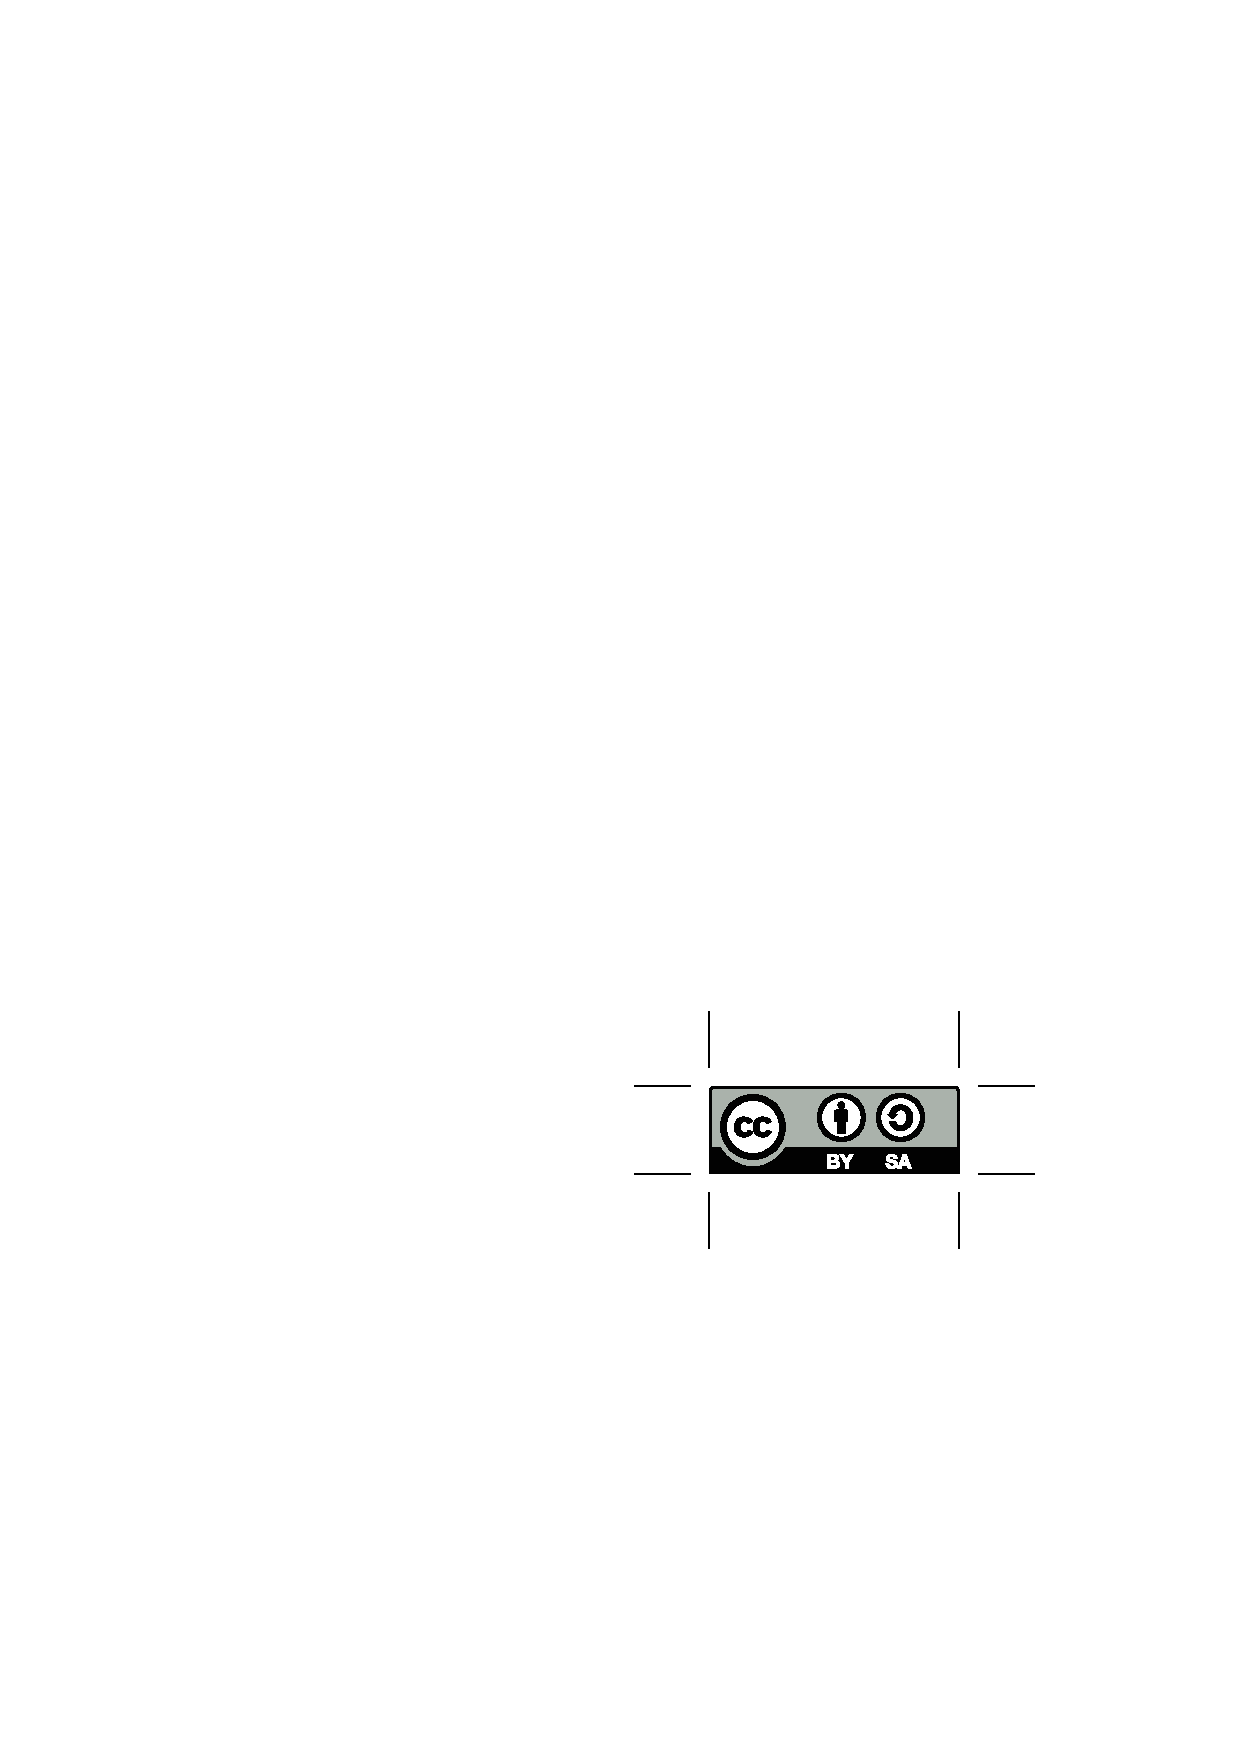
\includegraphics[scale=1]{by-sa} %
    \end{center} %
    
    Este trabajo titulado \emph{\thesisFlatTitle{}} por \thesisAuthor{}, se
    encuentra bajo la Licencia Creative Commons
    \href{http://creativecommons.org/licenses/by-sa/4.0/?ref=chooser-v1}%
    {Atribución-ShareAlike 4.0 International}.
    
    Para ver una copia de esta Licencia, visite
    \url{http://creativecommons.org/licenses/by-sa/4.0/}.\bigskip
    
    \copyright \the\year \hfill%
    \thesisAuthor \hfill%
    \thesisInstitution
  }
}

  
  % Hoja de depuración, con comandos definidos por la plantilla.
  % \phantomsection
\pdfbookmark[1]{Debug}{Debug}

Esta es una página de depuración, para ver todos los comandos
definidos en config.tex

De \verb+babel+ se obtiene que \verb+\tablename+ es \tablename.  Por
lo tanto, en esta versión se usará ``\latabla'' para denotar a cada
``\tabla''.  Ver \tabref{tab:comandostab} para la lista de comandos
existentes.



Este documento es elaborado por \thesisAuthorAddress~\thesisAuthor\
(\thesisAuthorShort) con carné \thesisAuthorTECID, para optar por el
título de \thesisAuthorDegree.

\genderAsesor\ \nameAsesor.

\genderLectorI\ \nameLectorI.

\genderLectorII\ \nameLectorII.

Titulo crudo:

\begin{center}
  \thesisTitle.  
\end{center}

Título aplanado:

``\thesisFlatTitle''.

Palabras clave: \thesisKeywords.

Fecha borrador: \thesisDraftDate

Fecha final: \thesisFinalDate





  
  \thispagestyle{empty}

\rule{10mm}{0pt}

\vfill

Declaro que el presente documento de tesis ha sido realizado enteramente
por mi persona, utilizando y aplicando literatura referente al tema e
introduciendo conocimientos y resultados experimentales propios.

En los casos en que he utilizado bibliografía he procedido a indicar las
fuentes mediante las respectivas citas bibliográficas.  En consecuencia,
asumo la responsabilidad total por el trabajo de tesis realizado y por
el contenido del presente documento.

\vspace*{8mm}

\begin{flushright}
  \thesisAuthor\par
  Cartago, \FechaFinal\par
  Céd: 1-1741-0734
\end{flushright}

\cleardoublepage

%%% Local Variables: 
%%% mode: latex
%%% TeX-master: "main"
%%% End: 

  %% -------------------------------------------------
  %% Acta y hoja del tribunal
  %%
  %% Asegúrse de que las fechas de defensa de tesis sean las que aparecen
  %% en las actas.
  
  %% Para la Licenciatura en Ingeniería Electrónica:

  %%   Acá se colocan las dos actas como plantillas para ser firmadas
  %%   por el tribunal.

  %%   El acta de aprobación, dependiendo del tribunal, puede dejarla
  %%   en blanco en la tesis, para que el tribunal firme la tesis completa
  %%   sobre esta acta, o, si el tribunal lo decide, extrae la hoja
  %%   para que sea firmada "caligráficamente" por los miembros del tribunal.
  %%   Al acta firmada, en formato PDF (ya sea firmado con tabletas gráficas o
  %%   en papel y escaneada) la integra al documento con el comando para incluir
  %%   el pdf directamente \includepdf{archivo} 
  %% ESTE ARCHIVO DEBE ELIMINARSE DE LA VERSIÓN FINAL

\thispagestyle{empty}

\begin{center}
  \begin{tabular}{c}
    \thesisInstitution \\
    \thesisDepartment \\
    Trabajo Final de Graduación \\
    Acta de Aprobación
  \end{tabular}
\end{center}

\vfill

\begin{center}
  \begin{tabular}{c}
    Defensa de Trabajo Final de Graduación \\
    Requisito para optar por el título de \thesisAuthorDegree\ en Electrónica\\
    Grado Académico de Licenciatura
  \end{tabular}
\end{center}

\vfill

%% \thesisAuthorAddress, \thesisAuthor y \thesisTitle están en main.tex
El Tribunal Evaluador aprueba la defensa del trabajo final de graduación
denominado \textsl{\thesisFlatTitle{}}, realizado por
%
\thesisAuthorAddress\ \thesisAuthor\ %
%
y, hace constar que cumple con las normas
establecidas por la \thesisDepartment{} del \thesisInstitution{}.

\vfill

\begin{center}
 Miembros del Tribunal Evaluador
\end{center}

\vfill

\begin{center}
  \begin{tabularx}{\textwidth}{cXc}
    \rule{0.45\textwidth}{0.5pt} && \rule{0.45\textwidth}{0.5pt} \\
    \nameLectorI                 && \nameLectorII \\
    \genderLectorI               && \genderLectorII
  \end{tabularx}
  
  \vspace{10mm}

  \begin{tabular}{c}
    \rule{0.45\textwidth}{0.5pt} \\
    \nameAsesor \\
    \genderAsesor
  \end{tabular}
\end{center}

\vfill

\begin{center}
  Cartago, \ifdraft{\thesisDraftDate}{\FechaFinal}\par
\end{center}

\cleardoublepage

%%% Local Variables: 
%%% mode: latex
%%% TeX-master: "main"
%%% End: 
  % Remover en versión final
  %\includepdf{acta_aprob_firmada} % Incluir el acta firmada acá.

  %% El acta de evaluación usualmente la extrae del documento y
  %% la entrega al tribunal para que sea firmada, y ellos la hacen
  %% llegar al profesor del curso de TFG.  Ese documento no
  %% debe aparecer en la tesis final, así que esta línea deberá
  %% comentarla en la versión final:
  %% ESTE ARCHIVO DEBE ELIMINARSE DE LA VERSIÓN FINAL


\thispagestyle{empty}

\begin{center}
  \begin{tabular}{c}
    \thesisInstitution \\
    \thesisDepartment \\
    Trabajo Final de Graduación \\
    Tribunal Evaluador \\
    Acta de Evaluación
  \end{tabular}
\end{center}

\vfill

\begin{center}
  \begin{tabular}{c}
    Defensa del Trabajo Final de Graduación \\
    Requisito para optar por el título de \thesisAuthorDegree\ en Electrónica\\
    Grado Académico de Licenciatura
  \end{tabular}
\end{center}

\vfill

%% Configurar todo en config.tex
\begin{center}

  Estudiante:%
  \qquad \textbf{\thesisAuthor}%
  \qquad Carné: \thesisAuthorTECID

  \vspace*{2ex}

  \setlength\tabcolsep{0pt}
  \begin{tabular}{p{.25\textwidth}p{.73\textwidth}}
    Nombre del proyecto: & \textsl{\thesisFlatTitle}
  \end{tabular}
\end{center}
\vspace{5mm}

\vfill

Los miembros de este Tribunal hacen constar que este trabajo final de
graduación ha sido aprobado y cumple con las normas establecidas por
la \thesisDepartment{} del \thesisInstitution{} y es merecedor de la
siguiente calificación:

\vfill

\begin{center}
  Nota del Trabajo Final de Graduación: \rule{25mm}{0.5pt}
\end{center}

\vfill

\begin{center}
 Miembros del Tribunal Evaluador
\end{center}

\vfill

% Defina con \setLector* en main.tex (líneas 87-89) los lectores y asesor
\begin{center}
  \begin{tabularx}{\textwidth}{cXc}
    \rule{0.45\textwidth}{0.5pt} && \rule{0.45\textwidth}{0.5pt} \\
    \nameLectorI                 && \nameLectorII \\
    \genderLectorI               && \genderLectorII
  \end{tabularx}
  
  \vspace{10mm}

  \begin{tabular}{c}
    \rule{0.45\textwidth}{0.5pt} \\
    \nameAsesor \\
    \genderAsesor
  \end{tabular}
\end{center}

\vfill

\begin{center}
  Cartago, \ifdraft{\thesisDraftDate}{\thesisFinalDate}\par
\end{center}

\cleardoublepage

%%% Local Variables: 
%%% mode: latex
%%% TeX-master: "main"
%%% End: 
   % >> Remover en versión final <<
    
  %% Para la maestría en electrónica:
  %%% ESTE ARCHIVO DEBE ELIMINARSE DE LA VERSIÓN FINAL

\thispagestyle{empty}

\begin{center}
  \begin{tabular}{c}
    \thesisInstitution \\
    \thesisDepartment \\
    Proyecto de Graduación \\
    Tesis de Maestría \\
    Tribunal Evaluador
  \end{tabular}
\end{center}

\vfill

Tesis de maestría defendida ante el presente Tribunal Evaluador como
requisito para optar por el grado académico de maestría, del
\thesisInstitution.

\vfill

\vspace*{20mm}
\begin{center}
 Miembros del Tribunal
\end{center}
\vspace*{8mm}

\vfill

\begin{center}
  \begin{tabularx}{\textwidth}{cXc}
    \rule{0.45\textwidth}{0.5pt} && \rule{0.45\textwidth}{0.5pt} \\
    \nameLectorI                 && \nameLectorII \\
    \genderLectorI               && \genderLectorII
  \end{tabularx}
  
  \vspace{10mm}

  \begin{tabular}{c}
    \rule{0.45\textwidth}{0.5pt} \\
    \nameAsesor \\
    \genderAsesor
  \end{tabular}
\end{center}

\vfill


Los miembros de este Tribunal dan fe de que la presente tesis de
maestría ha sido aprobada y cumple con las normas establecidas por la
\thesisDepartment.

\vfill

\begin{center}
  Cartago, \today\par
\end{center}

\cleardoublepage

%%% Local Variables: 
%%% mode: latex
%%% TeX-master: "main"
%%% End: 
  % Remover en versión final
  %%% ESTE ARCHIVO DEBE ELIMINARSE DE LA VERSIÓN FINAL


\thispagestyle{empty}

\begin{center}
  \begin{tabular}{c}
    \thesisInstitution \\
    \thesisDepartment \\
    Tesis de Maestría \\
    Acta de Evaluación
  \end{tabular}
\end{center}

\vfill

Tesis de maestría defendida ante el presente Tribunal Evaluador como
requisito para optar por el grado académico de maestría, del
\thesisInstitution.

\vspace*{15mm}

%% Configurar todo en config.tex
\begin{center}
  Estudiante: \thesisAuthor
\end{center}

\vfill

\begin{center}
  Nombre del Proyecto: \thesisFlatTitle}
\end{center}

\vspace*{20mm}
\begin{center}
 Miembros del Tribunal Evaluador
\end{center}
\vspace*{8mm}

\vfill

% Los nombres de lectores y asesor se definen en el archivo main.tex
\begin{center}
  \begin{tabularx}{\textwidth}{cXc}
    \rule{0.45\textwidth}{0.5pt} && \rule{0.45\textwidth}{0.5pt} \\
    \nameLectorI                 && \nameLectorII \\
    \genderLectorI               && \genderLectorII
  \end{tabularx}
  
  \vspace{10mm}

  \begin{tabular}{c}
    \rule{0.45\textwidth}{0.5pt} \\
    \nameAsesor \\
    \genderAsesor
  \end{tabular}
\end{center}

\vfill

Los miembros de este Tribunal dan fe de que la presente tesis de
maestría ha sido aprobada y cumple con las normas establecidas por la
\thesisDepartment.

\vfill

\begin{center}
  Nota final de la Tesis de Maestría: \rule{3cm}{0.5pt}
\end{center}
\vfill

\begin{center}
  Cartago, \today\par
\end{center}

\cleardoublepage

%%% Local Variables: 
%%% mode: latex
%%% TeX-master: "main"
%%% End: 
   % Remover en versión final
  %% -------------------------------------------------
  \chapter*{Resumen}
\thispagestyle{empty}

El resumen es la síntesis de lo que aparece en el resto del
documento. Tiene que ser lo suficientemente conciso y claro para que
alguien que lo lea sepa qué esperar del resto del trabajo, y se motive
para leerla completamente.  Usualmente resume lo más relevante de la
introducción y contiene la conclusión más importante del trabajo.

Es usual agregar palabras clave, que son los temas principales
tratados en el documento. El resumen queda fuera de la numeración del
resto de secciones.

Evite utilizar referencias bibliográficas, \tablas, o figuras en el
resumen.

\bigskip

%% Defina las palabras clave con defKeywords en config.tex:
\textbf{Palabras clave:} \thesisKeywords

\clearpage
\chapter*{Abstract}
\thispagestyle{empty}

Current advances in network speed, image processing, and digital technology have rendendered live video tools commonplace in professional, academic, and recreational contexts. Therefore, there has been increased interest in ensuring a high quality of experience (QoE) for these services.

Same content as the Spanish version, just in English.  Check
\href{https://deepl.com}{this site} for some help with the
translation.  For instance, the following is the automatic translation
from a previous version of the ``Resumen''.

The abstract is the synthesis of what appears in the rest of the
document. It has to be concise and clear enough so that someone
reading it knows what to expect from the rest of the text, and is
motivated to read it in full.  It usually summarizes the most relevant
parts of the introduction and contains the most important conclusion of
the work.

It is usual to add keywords, which are the main topics covered in the
document. The abstract is left out of the numbering of the rest of the
sections.

Avoid using bibliographical references, tables, or figures in the
abstract.

\bigskip

\textbf{Keywords:} word 1, word 2, 

\cleardoublepage

%%% Local Variables: 
%%% mode: latex
%%% TeX-master: "main"
%%% End: 

  \vspace*{0.4\textheight}
% No debe confundirse la dedicatoria con el agradecimiento.
% La dedicatoria solo tiene una línea corta de la persona a quien se dedica.

{\hfill{\Large{\emph{Dedicated to family, friends, and all that which keeps us sane}}}}

  \chapter*{Acknowledgements}
\thispagestyle{empty}

I thank my mom Maritza Badilla, my dad Ricardo Guindon, my sister Hazel, my brother David, the extended Guindon family, and the Monteverde community, which supplied the perfect environment for maximum development in both artistic endeavor and scientific enterprise.

I thank Elena, for sharing her support during the development of this project.

I thank my closest highschool friends Diego, Cristina, and Josue, for stubbornly distracting me from my research. I know you all were acting in my best interests, or so you all say.

I thank my closest college friend Emi, my close friends at the SeleHouse, my friends at Tec, and my friends at RidgeRun, which have all provided spaces where I've shared my research's progress.

I thank Marco Madrigal and Melissa Montero at RidgeRun, for contributing professional management over the dispTec project, as well as providing me with valuable lessons during one of the hardest points in my life.

I thank those brilliant minds I've worked with at RidgeRun, which have trained me in the art of developing all sorts of software shenanigans.

I thank Pablo Alvarado, for contributing his extensive personal expertise, his time and patience, his enthusiasm for understanding, his natural talent as an instructor, his steady push to bring out the most of me, and his nerdy jokes.

\vspace*{1cm}

\thesisAuthor

Cartago, \today

\cleardoublepage

%%% Local Variables: 
%%% mode: latex
%%% TeX-master: "paMain"
%%% End: 


  %----------------------------------------------------------------------------
  \frontmatter
  %----------------------------------------------------------------------------
  \pagestyle{fancy}
  \pagenumbering{roman}

  \pdfbookmark[1]{General Index}{General Index}

  \parskip0ex                           % space between paragraphs

  \tableofcontents                      % Table of contents
  \listoffigures                        % List of figures
  \listoftables                         % List of tables

\ifdraft{%
  % todo's                              % TODOs
  \listoftodo
}{%
}

  %% ---------------------------------------------------------------------------
%% paNotation.tex
%%
%% Notation
%%
%% $Id: paNotation.tex,v 1.15 2004/03/30 05:55:59 alvarado Exp $
%% ---------------------------------------------------------------------------

\cleardoublepage
\renewcommand{\nomname}{List of Symbols and Abbreviations}
\setlength{\nomitemsep}{-\parsep}

%%
% Commands required for the nomenclature groups
%
% There are following prefix forms:
%  a   abbreviation    \syma[key]{symbol}{description}
%  g   general         \symg[key]{symbol}{description}
%%

\renewcommand{\nomgroup}[1]{%
  \ifthenelse{\equal{#1}{G}}{\section*{\hspace*{-\leftmargin}General Notation}}{}%
  \ifthenelse{\equal{#1}{A}}{\section*{\hspace*{-\leftmargin}Abreviations and Acronyms}}{}%
}

\newcommand{\syma}[3][foo]{%
  \ifthenelse{\equal{#1}{foo}}%
  {\nomenclature[A]{#2}{#3}}{\nomenclature[A#1]{#2}{#3}}}
\newcommand{\symg}[3][foo]{%
  \ifthenelse{\equal{#1}{foo}}%
  {\nomenclature[G]{#2}{#3}}{\nomenclature[G#1]{#2}{#3}}}

%%
% Símbolos en la notación general
% (es posible poner la declaración en el texto
%%

\symg[yscalar]{$y$}{Scalar.}
\symg[xvector]{$\vct{x}$}{Vector. \newline\hspace{1mm}%
  $\vct{x}=\left[ x_1 \; x_2 \; \ldots \; x_n \right]^T =
  \begin{bmatrix}
    x_1 \\ x_2 \\ \vdots \\ x_n
  \end{bmatrix}$}

\symg[mmatrix]{$\mat{A}$}{Matrix. \newline\hspace{1mm}%
  $\mat{A} =
  \begin{bmatrix}
    a_{11} & a_{12} & \cdots & a_{1m}\\
    a_{21} & a_{22} & \cdots & a_{2m}\\
    \vdots & \vdots & \ddots & \vdots\\
    a_{n1} & a_{n2} & \cdots & a_{nm}\\
  \end{bmatrix}$}
  \symg[S]{$\set{S}$}{Set.}
  \symg[SN]{$\setN$}{Set of Natural Numbers.}
  \symg[SNE]{$\setN_{8-bit}$}{Set of 8-bit Natural Numbers. }

%%
% Algunas abreviaciones
%%

\syma{QoE}{Quality of Experience}
\syma{CPU}{Central Processing Unit}
\syma{GPU}{Graphics Processing Unit}
\syma{MPEG}{Moving Picture Experts Group}
\syma{PLDA}{Packet Loss Detection Algorithm}
\syma{NSGA-II}{Non-dominated Sorting Genetic Algorithm}
\syma{RDF}{Random Decision Forests}
\syma{VCL}{Video Coding Layer}
\syma{NAL}{Network Abstraction Layer}
\syma{SPS}{Sequence Parameter Set}
\syma{PPS}{Picture Parameter Set}
\syma{RTP}{Real-time Transport Protocol}
\syma{NCA}{Non-Concealed Artifact}
\syma{LSAA}{Low Spatial Activity Artifact}
\syma{HSAA}{High Spatial Activity Artifact}
\syma{TCA}{Temporally-Concealed Artifact}
\syma{PA}{Propagation Artifact}
\syma{RPD}{Random Packet Dropper}
\syma{ML}{Machine Learning}
\syma{SAT}{Summed-Area Table}
\syma{SSAT}{Squared Summed-Area Table}
\syma{ARM}{Acorn RISC Machine}
\syma{ITB}{In-the-Bag}
\syma{OOB}{Out-of-Bag}
\syma{TP}{True Positive}
\syma{TN}{True Negative}
\syma{FP}{False Positive}
\syma{FN}{False Negative}
\syma{dT2}{dispTEC2}
\syma{Art-FD}{Artifact Detector based on Random Decision Forests}
\syma{SIMD}{Singe-Instruction Multiple-Output}

\printnomenclature[20mm]

%%% Local Variables:
%%% mode: latex
%%% TeX-master: "paMain"
%%% End:
                    % Abbreviation

  \parskip1.3ex                         % space between paragraphs

  %----------------------------------------------------------------------------
  \mainmatter
  %----------------------------------------------------------------------------
  % where to look for graphics
  \graphicspath{{./}{./fig/}}
  %\pagenumbering{arab}

  % Main files
  %% ---------------------------------------------------------------------------
%% intro.tex
%%
%% Introduction
%%
%% $Id: intro.tex 1477 2010-07-28 21:34:43Z palvarado $
%% ---------------------------------------------------------------------------

\chapter{Introduction}
\label{chp:intro}

\section{Video artifacts in live video streaming}
\label{sec:intro_artifacts}

Modern streaming services are fundamental instruments in today's industries, institutions, and every day life. Live video conferencing and streaming services became the principal mediums of communication for a large sector of national and global society during the recent COVID-19 pandemic, thus exemplifying the crucial role that these services now have. Current advances in network speed and digital technology have enabled these services to become commonplace in professional, academic, and recreational contexts. Therefore, there has been increased interest in ensuring a high quality of experience (QoE) for these services.

One of the main issues affecting the QoE of video conferencing and live streaming services are video artifacts, as mentioned in \cite{Vranjes2018, Korhonen2018}. In \cite{Greengrass2009}, video artifacts, or simply artifacts, are defined as distortions in the images displayed to the user with respect to the original captured images. According to \cite{Vranjes2018}, artifacts are primarily caused by errors or loss of data in the transmission of the video over the network, or by losses caused during video compression.

Figure \ref{fig:lossy_system} illustrates the basic structure of a lossy video system. In order to send video through a network, the video gets encoded into network packets, then sent through a transmission channel where the losses occur, then decoded into video with artifacts. Figure \ref{fig:frame_comparison} compares two versions of the same image. Figure \ref{fig:frame_comparison.a} contains no video artifacts and Figure \ref{fig:frame_comparison.b} contains video artifacts due to packet loss.

\begin{figure} [!h]
  \centering
  
  \includegraphics{lossy_system}
  
  \caption{Lossy video transmission system}
  \label{fig:lossy_system}

\end{figure}

\begin{figure} [!h]
  \centering
  
  \begin{subfigure}[t]{0.49\textwidth}
    \centering
    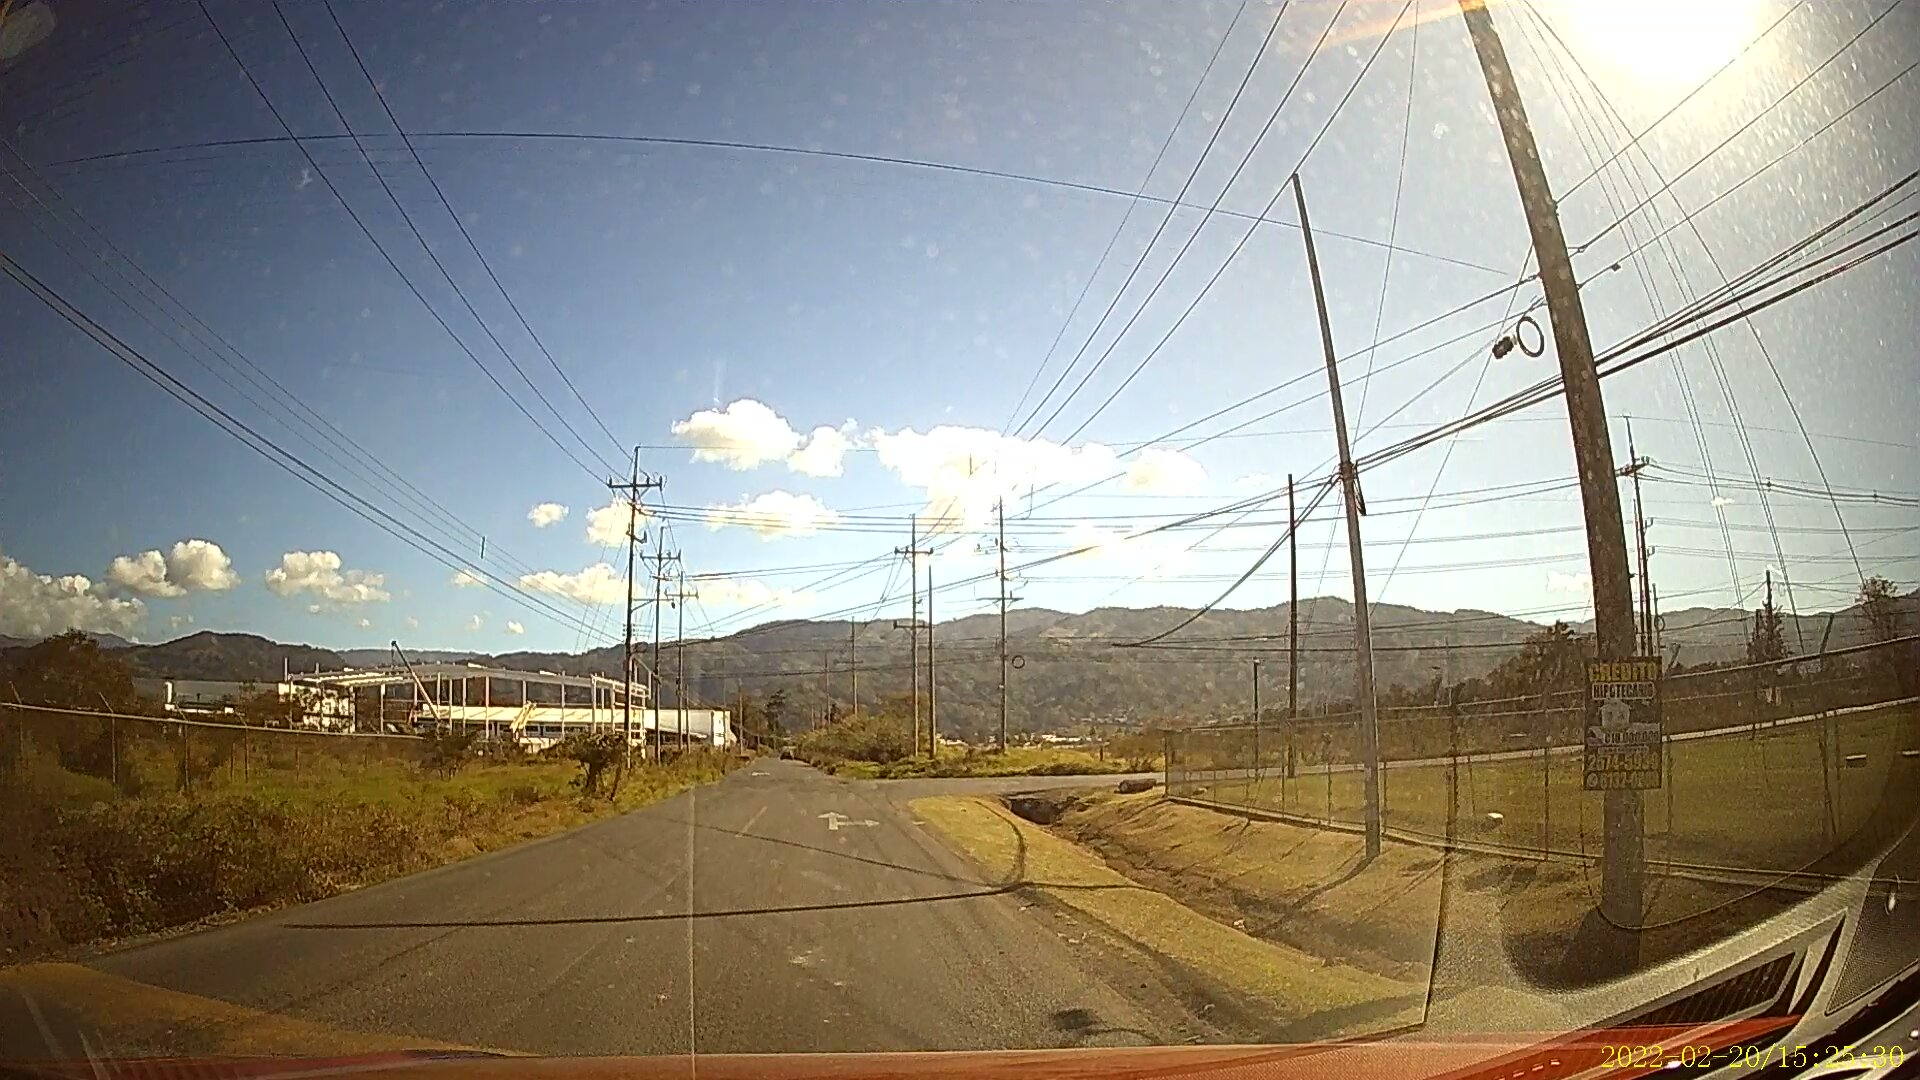
\includegraphics[width=\textwidth]{imgs_27}
    \caption{Frame with no video artifacts}
    \label{fig:frame_comparison.a}
  \end{subfigure}
  \hfill
  \begin{subfigure}[t]{0.49\textwidth}
    \centering
    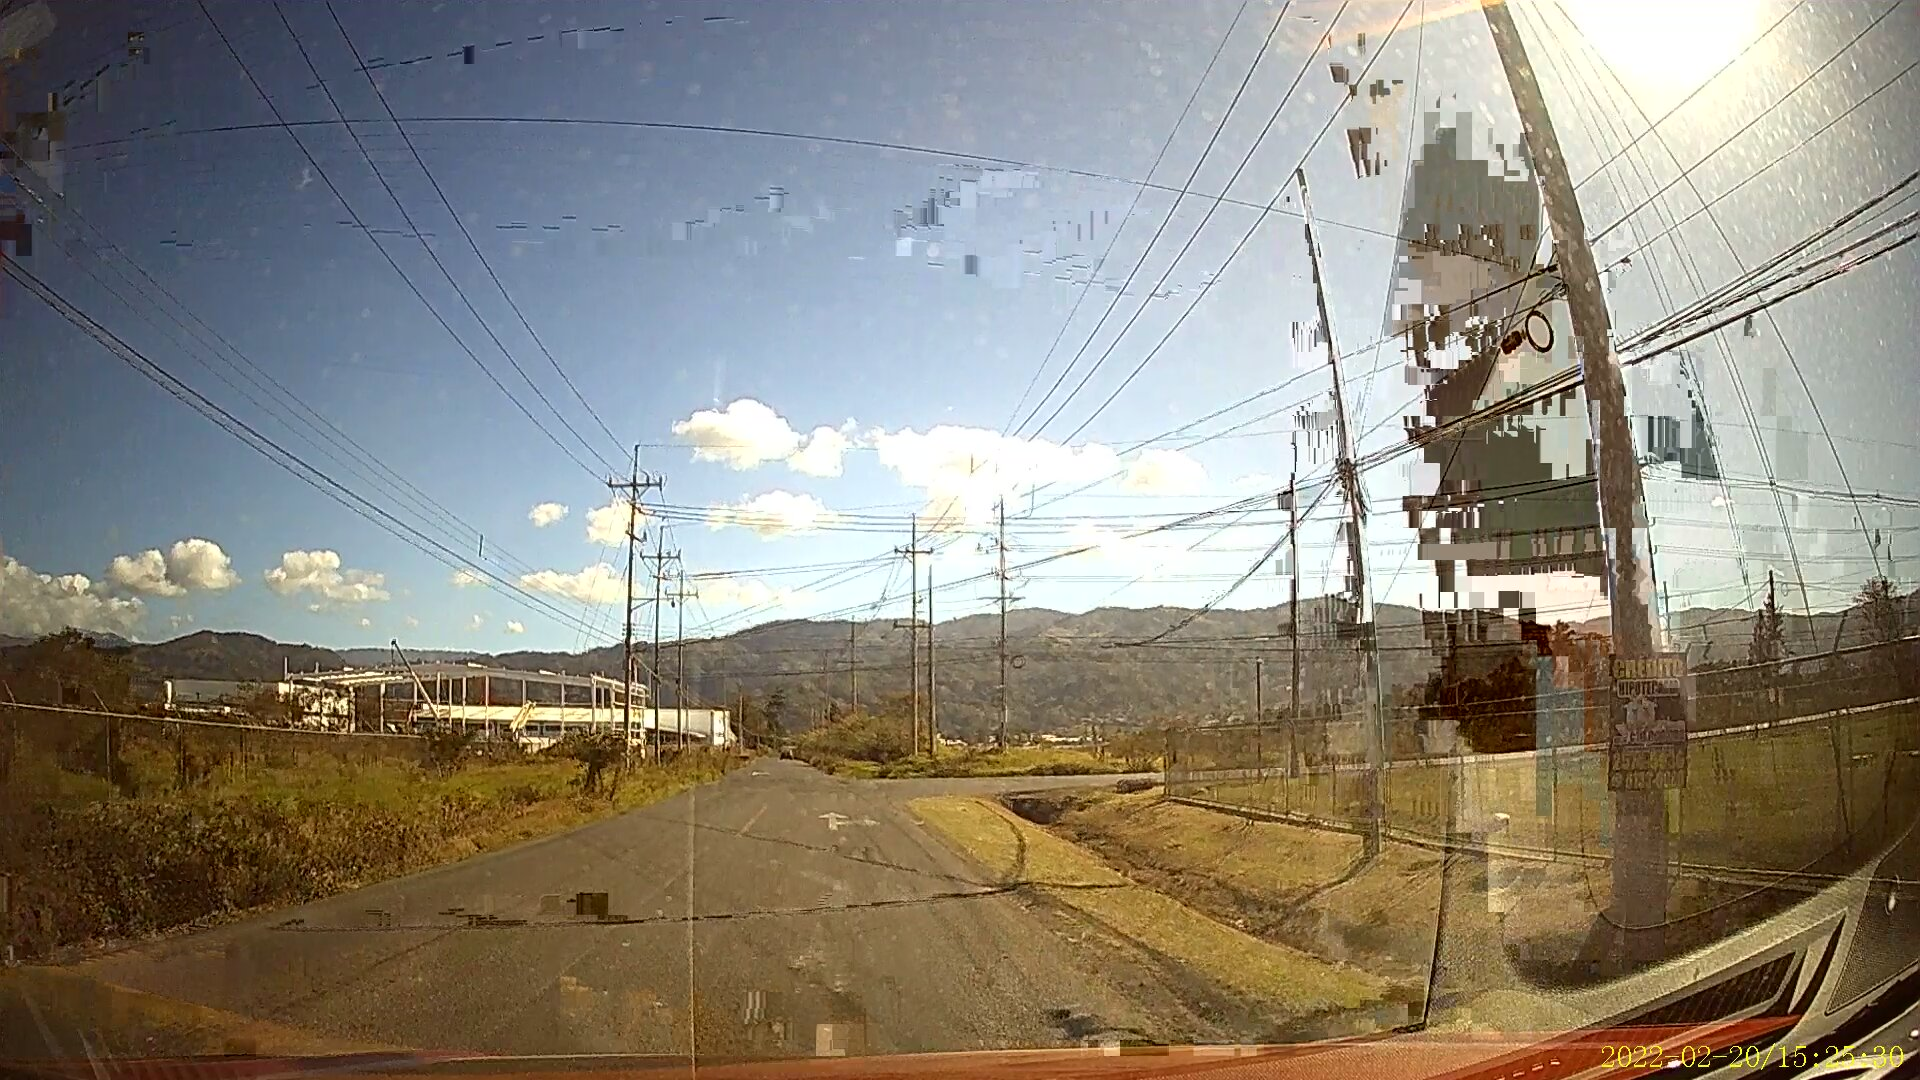
\includegraphics[width=\textwidth]{imgs_with_loss_27}
    \caption{Frame with video artifacts due to packet loss}
    \label{fig:frame_comparison.b}
  \end{subfigure}
  
  \caption{Comparison between a video frame with no artifacts and a video frame with artifacts caused by random h264 packet loss.}
  \label{fig:frame_comparison}

\end{figure}

There are methods to correct transmission errors in the transport layer or even in the video syntax layer, as mentioned in \cite{Sanyal2021}. In these cases, information is available on how the video packets are encoded, which simplifies the task of error detection and correction. When the user only has the decoded and decompressed information, it is necessary to use methods for artifact detection and correction that only have the raw video information, such as those of \cite{Vranjes2018, Sanyal2021,Goodall2019}. These methods are referred to as ``no-reference methods''.

Video artifacts result in loss of information from the original video. In video conferencing and live streaming applications, it is not possible to recover the lost data without affecting the user's QoE. In order to correct video artifacts, no-reference methods must infer the lost data. The process of restoring unknown areas of an image is called ``video inpainting'' \cite{Li2022, Zhou2021}. Video inpainting, or simply inpainting, is commonly used to remove the presence of objects in a video or image, but can be used to reconstruct areas of an image affected by video artifacts, as is done in \cite{Dong2023, Brenes2022}.

Modern inpainting algorithms use machine learning models. The inpainters of \cite{Li2022, Zhou2021, Liu2021} use ``transformers''. Transformers are machine learning models with outstanding results for signal restoration tasks, but they are slow and require signficant processing power. GPUs and other hardware accelerators are used in order to optimize the performance of these models.

Inpainting models such as \cite{Li2022} require binary masks to identify the areas to be reconstructed. For this reason, the location of video artifacts must be detected and binary masks must be generated and then used in the image restoration stage.

\cite{Greengrass2009, Glavota2016} classify the various types of artifacts generated by packet loss. These studies also describe the statistical properties of video artifacts. For example, certain video artifacts tend to have high-contrast vertical and horizontal edges that can be detected by high-pass filters. In the MPEG and H.26x video compression standards, the pixels of an image are grouped into ``macroblocks'', which are groups of $16 \times 16$ pixels in the image. Losses of packets containing macroblock information result in artifacts with well-defined edges \cite{Vranjes2019, Glavota2018}.

The artifact detection methods from \cite{Vranjes2018, Glavota2018} focus on filtering algorithms that do not involve machine learning. These methods can process standard definition video at 30 frames per second without GPU acceleration, but they oversimplify the characteristics of video artifacts and fail to perform well on the artifact detection task. The detectors of \cite{Goodall2019, Rajasekar2020} use neural network classifiers. These methods generalize better than filtering algorithms, but they require GPU accelerators in order to achieve comparable framerates with the filtering algorithms.

\section{The dispTEC2-2022 project}
\label{sec:intro_disptec}

During 2022, RidgeRun LLC and SIPLab developed the dispTEC2-2022 project with the objective of building a Video Restoration System using DeepLearning. The project was developed on Nvidia's Jetson TX2. This system has a 256 CUDA-core GPU, 4 ARM CPUs and 2 Denver CPUs. The development of the image restoration stage of dispTEC2-2022 is detailed in \cite{Brenes2022}.

The resulting system was capable of processing a video frame by frame. For each frame it could simulate randomly linear H264 packet losses, generate a binary detection mask based on the ground truth artifact measure, and then feed it along with the lossy frame into an inpainter transformer to produce a restored frame. \cite{Brenes2022} optimized the model with pytorch and CUDA, as well as a number of arquitectural optimizations. He finally concluded that the restoration system could reach a framerate from 0.8 to 1.67 frames per second on the Nvidia Jetson TX2.

However, this system cannot be used in practice because it relies on knowing the original frames in order to generate the binary detection masks. The system requires an artifact detector that can generate the masks from the lossy frames alone.

\section{The Artifact Detector Problem}
\label{sec:intro_problem}

The dispTEC2-2022 Video Restoration System concluded without a proper artifact detector. Part of dispTEC2-2022 entailed the search and development of an apropiate artifact detector for the system. The artifact detector was expected to run on the CPU alone, in order not to interfere with the CUDA-accelerated inpainting model. As a first approach, the dispTEC2-2022 team implemented the Packet Loss Detection Algorithm (PLDA) from \cite{Vranjes2018}. When testing the algorithm inside a gstreamer element, the algorithm could process a 720p video at $23,0$ frames per second.  After extensive testing of the algorithm using the Non-dominated Sorting Genetic Algorithm (NSGA-II), the dispTEC2-2022 team found no suitable parameters that allowed the detector to perform well on the detection task.

The dispTEC2-2022 team also developed a second artifact detection approach based on Random Decision Forests (RDF) \cite{Breiman2001}. In this approach, the RDF classifiers operated directly on each raw video frame and could achieve slightly better detection results than a random classifier. This classifier was trained on 200 frames from a training dataset containing only 2 video content types. When testing the RDF approach inside a gstreamer element, the algorithm could process 720p video at $26,6$ frames per second.

These results suggested that the RDF classifers were capable of learning artifact detection from the raw frame information. These results also suggested that the algorithm could be optimized to reach a framerate of $30$ frames per second.

\todo{Find PLDA framerate and metrics}
\todo{Find RDF framerate and metrics}

\section{Rangerx}
\label{sec:intro_detector}

The dispTEC2-2022 Video Restoration System is aimed at restoring video with artifacts frame by frame. Figure \ref{fig:restoration_system_overview} describes the general structure of the system and displays an example clip of an input frame with artifacts and the expected output clip from the system.

\begin{figure} [!h]
  \centering
  
  \includegraphics{video_inpainter_general}
  
  \caption{Video restoration system overview.}
  \label{fig:restoration_system_overview}

\end{figure}

In order to achieve this goal, Figure \ref{fig:restoration_system_steps} shows that the system is composed of the Artifact Detection System and the Inpainting System. The Artifact Detection System takes the frames with artifacts and generates binary detection masks. The Inpainting System takes the frame with artifacts and the detection masks and generates the restored video frames.

\begin{figure} [!h]
  \centering
  
  \includegraphics{video_inpainter_steps}
  
  \caption{Video restoration process. }
  \label{fig:restoration_system_steps}

\end{figure}

This project proposes Rangerx, a new Artifact Detection System. Rangerx aims to improve over the dispTEC2-2022 detection system by expanding the training dataset, redesigning and optimizing the feature extraction strategy, and replacing the RDF backend with the optimized Ranger C++ Core Library.

Random Decision Forests are subject to overfitting when training with small, highly self correlated datasets \cite{Breiman2001}. Rangerx expands the dataset with diverse video content in order to reduce the RDF detector overfitting.

The dispTEC2-2022 research found that RDF detectors could learn from raw image data. However, the feature extraction strategy can be improved by considering some of the statistical properties of artifacts described in \cite{Vranjes2019, Glavota2018}. Rangerx filters the raw image data to detect high contrast vertical and horizontal borders, then generates 132 statistical features from the filtered results.

Random Decision Forests agregate the results of a set of independent Decision Tree Classifiers. The dispTEC2-2022 RDF library ran the individual classifers consecutivelly. In contrast, the Ranger C++ Core Library runs the individual classifiers concurrently in seperate threads. Rangerx replaces the dispTEC2-2022 RDF backend with Ranger in order to improve the detection speed.

\section{Project objectives and document structure}
\label{sec:intro_objectives}

The aim of this project is to develop Rangerx, a real-time Artifact Detection System that can generate binary detection masks from video with artifacts. This system should improve over the dispTEC2-2022 system. This project focuses on video artifacts produced by decoding H264 packet loss. The system should run on an NVIDIA Jetson TX2 without using the GPU, which should be verified with CPU and GPU profiles. The training dataset should be expanded from the original 200 frames and 2 video content types to at least 18 video content types with 200 frames each. The new Artifact Detection System should achieve at least 70\% in both precision and recall detection metrics. The new system should provide a testing tool to verify these metrics. The new system should achieve a framerate of 30 frames per second. The new system should also provide a testing tool to verify the framerate.

The first milestone in the development of Rangerx is the expansion of the training dataset. This not only requires obtaining new video, but also requires procesing the videos to generate the ground truth binary masks that will be used as labels in the training procedure. \cite{Brenes2022} provides a similar tool, which can be used as a starting point. The final dataset should contain 18 video content types with at least 3 different illumination types.

The second milestone in the development of Rangerx is implementing the training procedure, the feature selection and the replacement of the RDF backend. These changes are aimed at improving the precision and recall detection metrics up to 70\%. Rangerx should provide a tool that can verify the detection performance against a test dataset.

The third milestone in the development of Rangerx is optimizing the feature selection and detection procedures in order to achieve real-time performance. Rangerx should provide a tool that can verify a framerate of 30 frames per second while testing the system on an input video.

The following chapters explore the project's main theoretical aspects, a detailed description of Rangerx and the final results. Chapter \ref{ch:marco} explores several theoretical concepts used in the development of Rangerx. Chapter \ref{ch:solucion} describes Rangerx in detail. Chapter \ref{chp:results} discusses Rangerx's final results. Chapter \ref{chp:conclusions} summarizes the project's main accomplishments, as well as future work related to Rangerx and dispTEC2-2022's Video Restoration System.

  \chapter{Theoretical Framework}
\label{ch:marco}

This work makes use of a number of key engineering concepts. First, this work studies the comparison between videos without artifacts and the same videos with artifacts generated from H264 packet loss. Section \ref{sec:h264} describes H264 video encoding. Section \ref{sec:h264_pl} describes the general characteristics of video artifacts caused by H264 packet losses. Section \ref{sec:simulation} describes packet loss simulation. Next, this work makes use of the RDF Classifier. Sections \ref{sec:classicalML} and \ref{sec:rdf_algorithm} explain Machine Learning and the RDF Classifier Algorithm, respectively. This work also makes use of mathematical concepts from Signal Processing. Section \ref{sec:2d_filter} explains the 2D Bi-linear High Pass Filtering algorithm. Section \ref{sec:sat_calc} explains the Summed-Area Table Algorithm. Finally, this work considers a series of hardware and software optimizations. Section \ref{sec:loop_unrolling} describes the software technique of loop fusion. Section \ref{sec:teo_multithreading} explains multithreading within the context of a multi-core machine. Section \ref{sec:tx2_simd} explains the characteristics of the TX2 target hardware.

\section{H264 Encoding}
\label{sec:h264}

H264 encoding compresses video into a series of Network Abstraction Layer (NAL) units \cite{h264}. These are either Video Coding Layer (VCL) units, which contain the compressed video data, or non-VCL units, which contain sequence (SPS) and picture (PPS) meta-data. These units are sent through a transmission channel in transport layer RTP packets \cite{Schulzrinne2003} from one end-point machine to another. An H264 bitstream refers to complete stream of packets corresponding to an input video source. The H264 decoding algorithm is used to recreate the video at the receiving end-point with varying degrees of compression distortion. Under certain encoding settings, H264 encodes and decodes Digital Satellite TV quality video at 1.5 megabits per second \cite{Jesup2011}.

Some features of H264 encoding are frame color subsampling, integer discrete cosine transform for intra-picture compression, and inter-picture prediction \cite{h264}. H264 makes use of video frames with I420 color subsampling, which compresses each frame to half the original size by separating the luma and chroma components of an image, then subsampling the chroma components by a factor of 2 in each dimension.

\todo{I420 Layout Diagram}

The Integer Discrete Cosine Transform is used to compress video frames by only considering the low frequency components of an image. These components are then used with the Inverse Integer Discrete Cosine Transform to recreate the image with minimal distortion. Within the context of video encoding, image compression is sometimes refered to as spatial or intra-picture compression.

H264 inter-picture prediction allows to compress some video frames with respect to previous or future frames by motion estimation and motion compensation. Motion estimation compares pixel blocks, computes block differences, and generates set of motion vectors. These vectors allow predicted frames to be constructed from previous frames. By using 6-tap filtering (a kind of 6th order digital filter) the frame prediction can interpolate block motion and reduce artifacts caused by compression.

Encoded video frames are classified into 3 categories: I-frames, P-frames, and B-frames. I-frames only use spatial compression and are used as references for P-frames and B-frames. P-frames only store motion predictions with respect to previous I-frames or P-frames. B-frames use motion predictions with respect to previous I-frames or P-frames, as well as following I-frames or P-frames. The distance between reference frames (I-frames or P-frames) and the distance between I-frames are parameters that affect the bitrate of the encoded video.

\todo{H264 frame types diagram}

\section{Types of Artifacts caused by H264 Packet Loss}
\label{sec:h264_pl}

H264 and MPEG-2 (another video encoding algorithm) differ in may ways. However, they share the same types of artifacts caused by packet loss. MPEG-2 artifacts are classified in \cite{Greengrass2009} as slice errors, blocking or pixelation errors, ghosting, and freeze frames.

Slice errors occur when H264 packets corresponding to complete rows of an image are dropped. These losses mostly occur in I-frame packets and cause strips of the video to appear distorted. Blocking or pixelation errors occur within I-frames or certain P-frames. These losses can either appear as black macroblocks or as macroblocks that belong to previous frames. Ghosting occurs when errors in reference frames are propagated by following P-frames or B-frames. These errors produce chaotic distortions and may spread over a frame region. These errors usually disappear at the next I-frame. Freeze frames happen when complete frames are lost. This occurs when H264 header packets are lost. Header packets contain meta-data that describe general frame characteristics. These packets are crucial to reconstruct the frame from the encoded information. Losses in I-frame headers cause significant artifacts for an entire frame sequence until the arrival of the next I-frame.

Additionally \cite{Glavota2016} classifies H264 packet loss artifacts in two main categories: rectangular artifacts and irregular artifacts. They then define a series of artifact types that fall into these two categories. Non-concealed Artifact (NCA) are rectangular artifacts that appear black in the frame. These artifacts usually follow macroblock borders. Low spatial activity artifact (LSAA) are rectangular artifacts that contain some details from the surrounding frame region. High spatial activity artifact (HSAA) are rectangular artifacts that contain internal borders and considerable detail from the surrounding frame region. Temporally-concealed artifacts (TCA) are either rectangular or irregular artifacts that contain information from previous frames. Propagation artifacts (PA) are irregular artifacts caused by motion prediction on rectangular artifacts in previous frames. These artifacts cause dramatic distortions and do not follow predictable boundaries.

\section{Packet Loss Simulation}
\label{sec:simulation}

\def\N8{\setN_\text{8-bit}}

Mathematically, a video \mat{V} is a 4-tensor of pixel values $p$ and dimensions $N$, $C$, $H$, and $W$. $N$ is the number of video frames in \mat{V}. A video frame $\mat{F}_n$ at time $n$ has width $W$, height $H$, and number of color channels $C$. A pixel value is an unsigned positive 8-bit integer, which is modeled as

\begin{equation}
  \label{eq:PV}
  p \in \N8
\end{equation}

where

\begin{equation}
  \label{eq:N8}
  \N8 = \{ n \in \setN \mid 0 \le n < 2^8  \}
\end{equation}

\def\VA{\mat{V}_A}
\def\VB{\mat{V}_B}

A video with artefacts $\VA$ is generated from a base video $\VB$ (without artifacts) using

\def\DEC{D_{H264}}
\def\RPD{\text{RPD}_{P_d}}
\def\ENC{E_{H264}}
\begin{equation}
  \label{eq:V_A}
  \VA = \DEC\left(\RPD\left(\ENC\left(\VB\right)\right)\right)
\end{equation}

\def\ph264{\text{P}_{\text{H264}}}

where $\ENC$ and $\DEC$ are the H264 encoding and decoding algorithms, respectively \cite{h264}. $\RPD$ is the Random H264 Packet Dropper with constant drop probability $P_d$. The $\RPD$ model is

\def\H264PV{\vct{P_\text{H264}}}
\def\XPD{\vct{X_{P_d}}}
\begin{equation}
  \label{eq:RPD}
  \left[\RPD(\H264PV)\right]_{i} = \H264PV[i]\cdot\XPD[i]
\end{equation}

where $\H264PV$ is a vector consisting of the encoded H264 Packets and $\XPD[i]$ is a Bernoulli distributed random vector such that

\begin{equation}
  \label{eq:XPDSET}
  \XPD[i] \in \{0,1\}
\end{equation}

and

\begin{equation}
  \label{eq:XPDPROB}
  P\left(\XPD[i]=1\right)=P_d
\end{equation}

\section{Machine Learning}
\label{sec:classicalML}

Machine Learning (ML) is a field of study and development focused on designing algorithms that learn from a dataset and automatically improve some performance metric \cite{Jordan2015}. ML algorithms are described as functions with adjustable parameters. While training an ML model with a given dataset, these parameters are automatically adjusted or ``learned'' such that they improve at a chosen performance metric. A performance metric encodes the task to be performed by a given algorithm. For example, error detection is a classification problem, since input data can fall into an \emph{error} category or a \emph{non-error} category. An error detection performance metric then considers either high or low performance if the algorithm classifies the input data correctly or incorrectly, respectively.

Three major paradigms of ML are supervised, unsupervised, and reinforcement learning. Supervised learning refers to ML algorithms that learn on a dataset where the desired output for each input is known. In these algorithms, the training data takes a form of an input-output pair. Unsupervised learning analyzes ML algorithms that learn from the input data alone. Reinforcement learning determines policies that agents can use to continuously improve on a reward metric within a controled environment.

A popular machine learning approach is deep learning. Deep learning methods use artificial neural networks and backpropagation at their core. These methods can achieve high performance on a variety of tasks, provided a large enough training dataset. These methods also benefit from their capacity to automatically determine features from the input data that improve their performance metrics.

There are machine learning algorithms besides neural networks. In this work, these approaches are considered Classical Machine Learning. The RDF classifier used in this work is a classical approach. RDF classifiers use a separate input feature selection strategy to perform well. For instance, the RDF classifier used in \cite{Sewak2018} outperforms a deep learning model at malware detection. This RDF classifier uses a Variance Threshold technique for feature selection.

\subsection{Random Decision Forests}
\label{sec:rdf_algorithm}

Random Decision Forests (RDF) are widely used classifiers. Some important milestones in the development of Random Decision Forests are \cite{Freund1996, Freund1996, Ho1998,Bauer1999, Breiman1999, Breiman2000, Breiman2001, Breiman1996, Pedregosa2011}. The algorithm was first completely described mathematically by Breiman in 2001, even though the algorithm had already been around since the late 90s.

The RDF classification or prediction algorithm aggregates the results from an ensemble of Decision Tree Classifiers \cite{Quinlan1986,Quinlan1987}. This ensemble is called a forest and the number of classifiers in the forest is $N_T$. A tree classifier is modeled by a root node that branches out into a left child node and a right child node. Each child node recursively branches out in binary fashion until they reach terminal ``leaf'' nodes. The non-terminal nodes store a feature index $i$, threshold $T_{H}$ pair. Leaf nodes store an output category. In the example of error detection, each leaf node is either assigned to the \emph{error} category or the \emph{non-error} category. To perform a prediction on an input feature vector $\vct{x}$, a tree evaluates the vector at the root node, and then recursively evaluates the vector on a single child node until a leaf node is reached. A node with a stored $(i,T_H)$ pair evaluates a vector by comparing its $i$-th component with $T_H$. If the vector value is less than the threshold, the tree evaluates the left child node. Otherwise, the tree evaluates the right child node. The prediction result is the category assigned to the final leaf node.

Figure \ref{fig:rdf_example} displays an example of decision tree classification. The input $\vct{x}$ has two features of values 3 and 6. The root node compares the first feature against a threshold of 1. Since 3 is greater than 1, the tree evaluates the right child node. This node compares the second feature against a threshold of 7. Since 6 is less than 7, the tree evaluates the left child node. This node compares the first feature against a threshold of 4. Since 3 is less than 4, the tree evaluates the left child node. Since this node is a leaf node, the output $y$ is set to the leaf node's value of 1.

\begin{figure} [!h]
  \centering
  \includegraphics{rdf_trainer}
  \caption{Example of decision tree classification}
  \label{fig:rdf_example}
\end{figure}

The RDF training algorithm generates the forest structure used in the prediction algorithm from a dataset of input-output pairs. The algorithm trains each tree in the forest on a different bootstrapped dataset. A bootstrapped dataset is a random sample of the input dataset with the possibility of data replacement. The method of training an ensemble of classifiers, each with a different bootstrapped dataset, and then aggregating the classifier results during prediction is called bagging \cite{Breiman1996}.

Each tree in the forest trains by starting at the root node and recursively subpartitioning the dataset at each node until a minimum dataset size or a maximum tree depth $D_T$ is reached. Each node splits its dataset subpartition by testing a finite random set of index and threshold pairs on the dataset and determining the pair with the largest information gain. The algorithm then assigns the index and threshold pair with the highest information gain to the node.

The information gain of an input index and threshold pair for a given dataset is calculated by the gini index (also called the gini impurity or gini criterion) \cite{Gini1936,Gelfand1991}. Given a dataset $\set{D}$ of input-output pairs, the Gini impurity is calculated as
%
\begin{equation}
  \label{eq:gini}
  Gini(\set{D}) = 1 - \sum_{i=1}^{k} p_i^2
\end{equation}
%
where each dataset output belongs to one of $k$ classes and $p_i$ is the probability that an output belongs to the $i$-th class.

An index-threshold pair $(i,T_H)$ partitions $\set{D}$ into subsets $\set{D}_1$ and $\set{D}_2$. $\set{D}_1$ consists of input-output pairs where inputs at index $i$ are less than $T_H$. $\set{D}_2$ consists of the remaining input-output pairs from $\set{D}$. The Gini impurity of the dataset split is
%
\begin{equation}
  \label{eq:gini}
  Gini_{(i,T_H)}(\set{D}) = \frac{N_1}{N}\cdot Gini(\set{D}_1) + \frac{N_2}{N}\cdot Gini(\set{D}_2)
\end{equation}
%
where $N$ is the size of $\set{D}$, $N_1$ is the size of $\set{D}_1$, and $N_2$ is the size of $\set{D}_2$.

Bootstrapping introduces randomization into the training of the model. Additionally, the RDF algorithm trains each tree on a different random subset of the input indices and thresholds. These three randomization mechanisms allow the RDF algorithm to perform well on classification tasks without overfitting to the training data.

\section{2D High Pass Filter}
\label{sec:2d_filter}

2D high pass filters are used for border detection and the computation of features to detect video artifacts \cite{Glavota2016, Vranjes2018}. The filter used in this work applies an absolute horizontal and vertical adjacent pixel difference over an input frame $\mat{F}$. The horizontal and vertical filters are modeled by
%
\def\HFF{\text{HFF}}
\def\VFF{\text{VFF}}
\begin{equation}
  \label{eq:hf}
  \left[\HFF(\mat{F})\right]_{i,j} =
  \begin{cases}
    + \mat{F}[i,j] - \mat{F}[i-1,j] & \text{if \hspace{0.5cm}} \mat{F}[i,j] \ge \mat{F}[i-1,j] \\
    - \mat{F}[i,j] + \mat{F}[i-1,j] & \text{otherwise}
  \end{cases}
\end{equation}
%
and
%
\begin{equation}
  \label{eq:vf}
  \left[\VFF(\mat{F})\right]_{i,j} =
  \begin{cases}
    + \mat{F}[i,j] - \mat{F}[i,j-1] & \text{if \hspace{0.5cm}} \mat{F}[i,j] \ge \mat{F}[i,j-1] \\
    - \mat{F}[i,j] + \mat{F}[i,j-1] & \text{otherwise}
  \end{cases}
\end{equation}
%
respectively. The filtered frames have pixels with larger values in high contrast image locations and can be used to detect borders within frames. Another border detection method is the Sobel Filter \cite{Korhonen2018}, but this method requires more computation.

High contrast artifact borders produce larger filtered values. Furthermore, these larger valued filtered borders lie close to the macroblock borders at a higher frequency than in the inner macroblock area due to the frequency of packet losses in I-frames \cite{Glavota2016, Vranjes2018}. The sum of the filtered values around macroblock borders provides useful information that is used to detect the presence of artifacts.

\section{Summed-Area Tables}
\label{sec:sat_calc}

Summed-Area Tables (SAT) allow the efficient computation of image frame subregion pixel sums \cite{Crow1984}. For an input frame $\mat{F}$ each new value SAT$[i,j]$ is calculated as:
%
\def\SAT{\text{SAT}}
\begin{equation}
  \label{eq:satgen}
  \left[\SAT(\mat{F})\right]_{i,j}=\mat{F}[i,j]+\SAT[i-1,j]+\SAT[i-1,j]-\SAT[i-1,j-1]
\end{equation}
%
Each value of $\SAT[i,j]$ represents the summed pixels in the rectangular area from $\mat{F}[0,0]$ to $\mat{F}[i,j]$. Figure \ref{fig:sat} illustrates the terms in \equ{eq:satgen}.

\begin{figure} [!h]
  \centering
  \includegraphics{sat}
  \caption{SAT construction on position $(i,j)$.}
  \label{fig:sat}
\end{figure}

The main advantage of using SATs is to efficently calculate frame subregion sums by
%
\begin{equation}
  \label{eq:satuse}
  A_r(i,j,H_r,W_r)=\text{SAT}[i,j]-\text{SAT}[i-H_r,j]-\text{SAT}[i,j-W_r]+\text{SAT}[i-H_r,j-W_r]
\end{equation}
%
where the area $A_r$ with bottom right pixel $(i,j)$, height $H_r$, and width $W_r$ is computed from the arithmetic operation of four SAT values.

Figure \ref{fig:satuse} illustrates the terms from \equ{eq:satuse}.
\begin{figure} [!h]
  \centering
  \includegraphics{satuse}
  \caption{Subregion sum calculation using SAT.}
  \label{fig:satuse}
\end{figure}

A Squared SAT (SSAT) is calculated by
%
\def\SSAT{\text{SSAT}}
\begin{equation}
  \label{eq:ssat}
  \left[\SSAT(\mat{F})\right]_{i,j}=\mat{F}^2[i,j]+\SSAT[i-1,j]+\SSAT[i-1,j]-\SSAT[i-1,j-1]
\end{equation}
%
and is used to efficiently calculate means and variances \cite{Crow1984}.

The mean of a frame subregion $\mu_r$, with pixel sum $A_r$, height $H_r$, and width $W_r$ is calculated as
%
\begin{equation}
  \label{eq:mu_r}
  \mu_r = \frac{A_r}{H_r\cdot W_r}
\end{equation}
%
and given the squared pixel sum $SA_r$ for the same subregion, the variance is calculated as
%
\begin{equation}
  \label{eq:var_r}
  \sigma^2_r = \frac{SA_r - A^2_r}{H_r\cdot W_r}
\end{equation}
%

\section{Loop Fusion}
\label{sec:loop_unrolling}

Loop fusion is a method to improve an algorithm's performance \cite{Kennedy1994}. Software loops translate into CPU branching instructions. In modern segmented architectures, branching instructions hinder instruction-level parallelism since new instructions cannot be loaded until the outcome of the branching operation is known. Branch prediction partially improves the hardware performance. However, by merging software loops into a single loop, the use of branching operations is reduced and the performance improves.

\section{Multithreading}
\label{sec:teo_multithreading}

Multithreading allows a machine to run several tasks simultaneously \cite{Saavedra1990}. Each task runs on a thread. This technique improves the efficiency and performance of a program. On a machine with multiple cores, each thread runs on an indepedent core at maximum frequency. It is possible to run multiple threads within a single core, however the core has to switch between the threads, which reduces the performance improvement provided by multithreading.

\section{The Nvidia Jetson TX2 System}
\label{sec:tx2_simd}

The Nvidia Jetson TX2 Embedded System \cite{tx2} provides 4 ARM processors, 2 Denver cores which are not generally used, and a 256-core GPU. With these resources, the TX2 can run a wide range of accelerated machine learning algorithms. For this work, only the CPU resources are considered. The TX2 CPU has four ARM cores that run at 2 GHz.

The ARM CPU cores provide the Neon Single-Instruction Multiple-Data (SIMD) extension. SIMD allows repetitive data operations to be parallelized within a single CPU, which improves the time performance of a program.

  \chapter{The Rangerx Artifact Detection System}
\label{ch:solucion}

\section{Artifact Detection System Structure}
\label{sec:sol_struct}

The Artifact Detection System generates detection masks from frames with artifacts. These masks are white on macroblocks which contain artifacts and black on the remaining artifacts. Figure \ref{fig:detector_overview} illustrates the input frame with artifacts, which is processed by the system, and finally produces the detection masks.

\begin{figure} [!h]
  \centering
  
  \includegraphics{detector_general}
  
  \caption{General Artifact Detection System Overview. }
  \label{fig:detector_overview}

\end{figure}

In order to achieve this, the Artifact Detection System must first extract features from the input frame. These features become the inputs to the RDF Classifier. The RDF Classifier outputs a prediction vector. The prediction vector is then mapped to the binary mask output. Figure \ref{fig:detector_steps} illustrates these steps.

\begin{figure} [!h]
  \centering
  
  \includegraphics{detector_steps}
  
  \caption{Artifact Detection process. }
  \label{fig:detector_steps}

\end{figure}

This structure was used in the dispTEC2-2022 RDF system. The Rangerx system maintains this structure and improves over the previous system by 

\subsection{The Feature Extractor}
\label{sec:sol_features}

The feature extractor

\begin{figure} [!h]
  \centering
  
  \includegraphics{extractor_steps}
  
  \caption{Feature extraction process. }
  \label{fig:extractor_steps}

\end{figure}

\subsection{The RDF Classifier}
\label{sec:sol_rdf}

\subsection{The Mask Generatorr}
\label{sec:sol_maskgen}

\section{Training}
\label{sec:sol_}



\section{Testing}
\label{sec:intro_problem}

\section{Video Artifact Detection}
\label{sec:intro_problem}

\section{Video Artifact Detection}
\label{sec:intro_problem}

\section{Video Artifact Detection}
\label{sec:intro_problem}

  \chapter{Resultados y análisis}

En este capítulo se exponen los diseños experimentales realizados para
comprobar el funcionamiento correcto del sistema. Por ejemplo, si se
realiza algún sistema con reconocimiento de patrones, usualmente esta
sección involucra las llamadas \emph{matrices de confusión} donde se
compactan las estadísticas de reconocimiento alcanzadas. En circuitos
de hardware, experimentos para determinar variaciones contra ruido,
etc. También pueden ilustrarse algunos resultados concretos como
ejemplo del funcionamiento de los algoritmos. Puede mostrar por medio
de experimentos ventajas, desventajas, desempeño de su algoritmo, o
comparaciones con otros algoritmos.

Recuerde que debe minimizar los ``saltos'' que el lector deba hacer en
su documento. Por tanto, usualmente el análisis se coloca junto a
tablas y figuras presentadas, y debe tener un orden de tal modo que se
observe cómo los objetivos específicos y el objetivo general del
proyecto de tesis se han cumplido.

  \chapter{Conclusiones}
\label{chp:conclusions}

One improvement is the expansion of the training dataset to 12.7 million samples, from the previous 2.3 million samples. These new samples are categorized into 19 different video content types, which improves over the previous 2 categories. Rangerx also implements a new feature extraction strategy, which improves detection performance to almost 0 Out Of Bag (OOB) prediction error over the complete dataset. Finally, Rangerx improves over the previous RDF Detector by optimizing the feature extraction and modifying the RDF backend to the Ranger C++ Core Library.

Las conclusiones no son un resumen de lo realizado sino a lo que ha llevado el
desarrollo de la tesis, no perdiendo de vista los objetivos planteados desde
el principio y los resultados obtenidos.  En otras palabras, qué se concluye o
a qué se ha llegado después de realizado la tesis de maestría.  Un error
común es ``concluir'' aspectos que no se desarrollaron en la tesis, como
observaciones o afirmaciones derivadas de la teoría directamente.  Esto último
debe evitarse.

Es fundamental en este capítulo hacer énfasis y puntualizar los
aportes específicos del trabajo.

Es usual concluir con lo que queda por hacer, o sugerencias para mejorar los
resultados.



  %----------------------------------------------------------------------------
  % literature in bibtex way:
  % \bibliographystyle{sty/plainurl} % for english documents
  % \bibliography{literatura}
  % literature in biblatex/biber way
  \printbibliography[title={Bibliografía},heading=bibintoc]
  %----------------------------------------------------------------------------

  %----------------------------------------------------------------------------
  \appendix
  %----------------------------------------------------------------------------

  \chapter{Anexos}
\label{apx:apendice}
\textbf{Exposición de anteproyecto:} \url{https://www.youtube.com/watch?v=7vysEp_0tss}
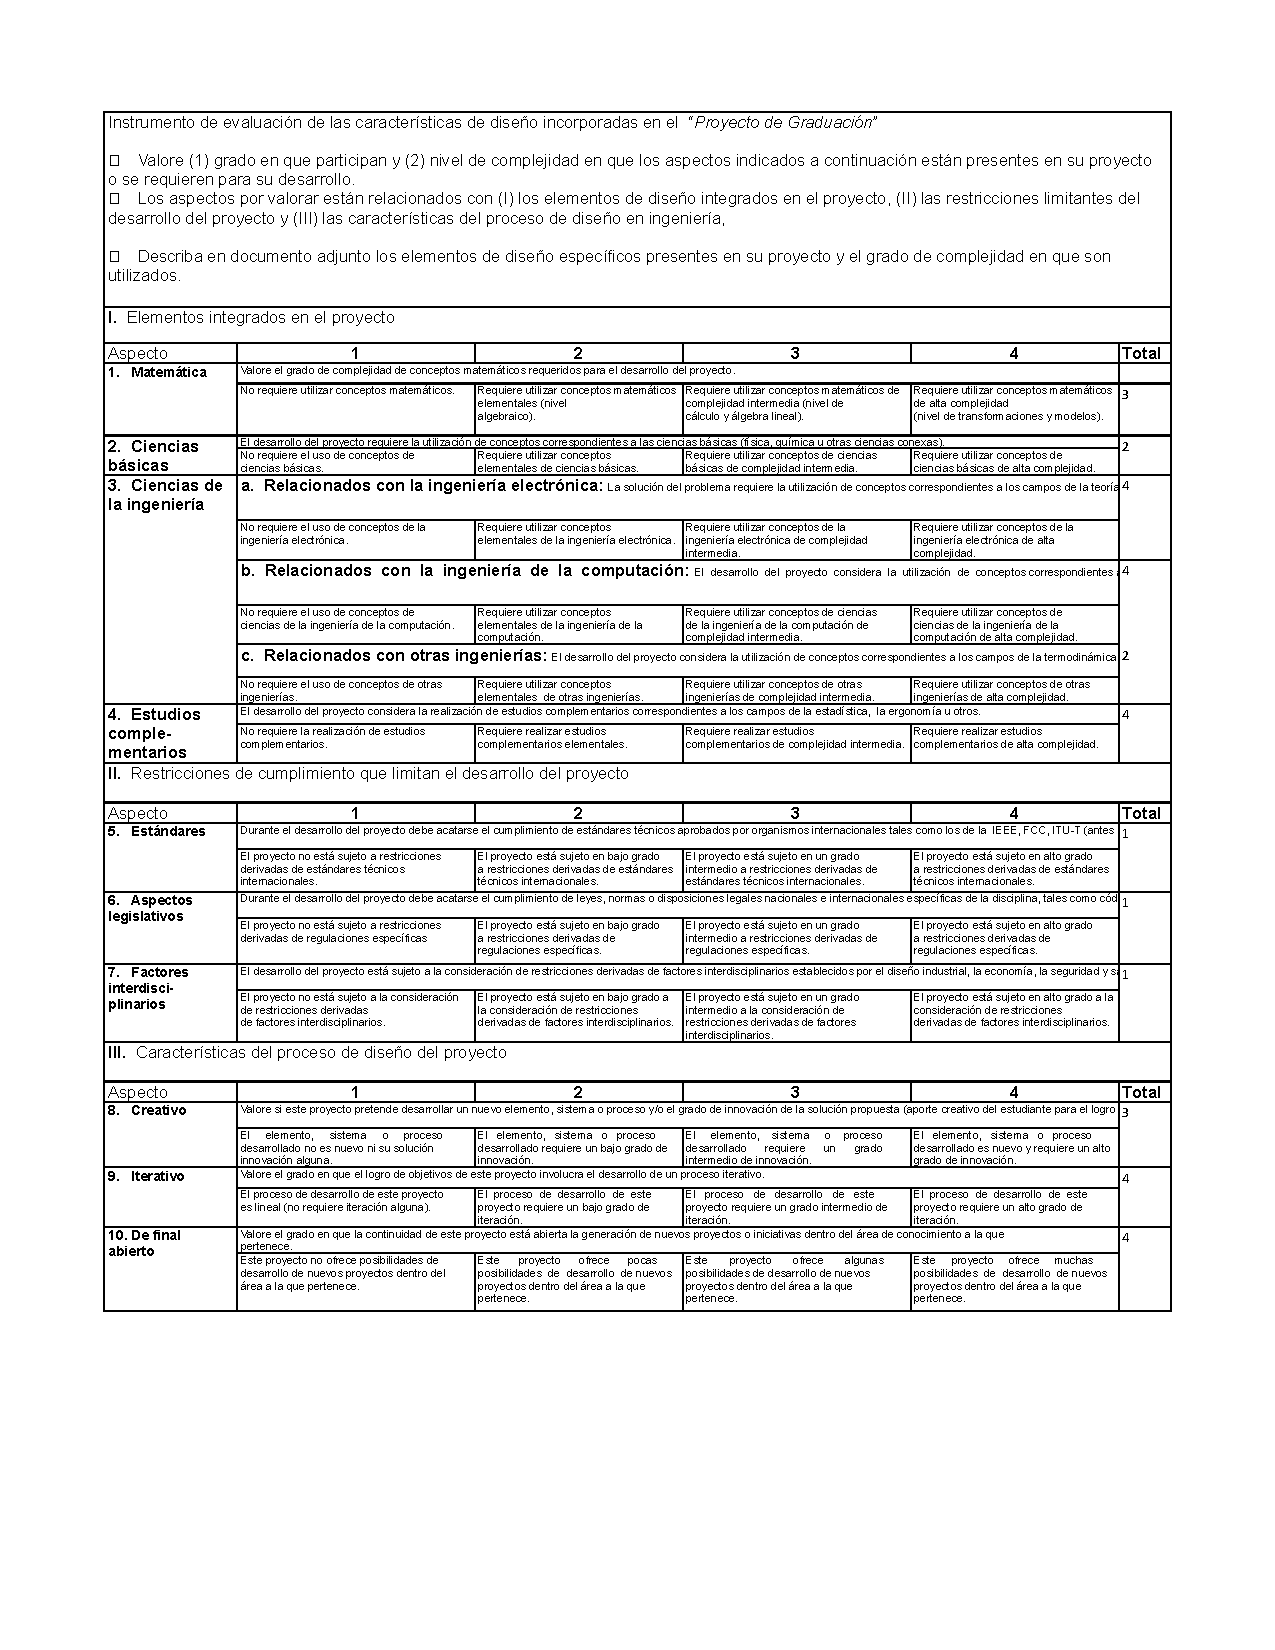
\includepdf[scale=1, offset=3cm -4cm, pagecommand={\textbf{Anexo A}}]{caracteristicas_proceso.pdf}
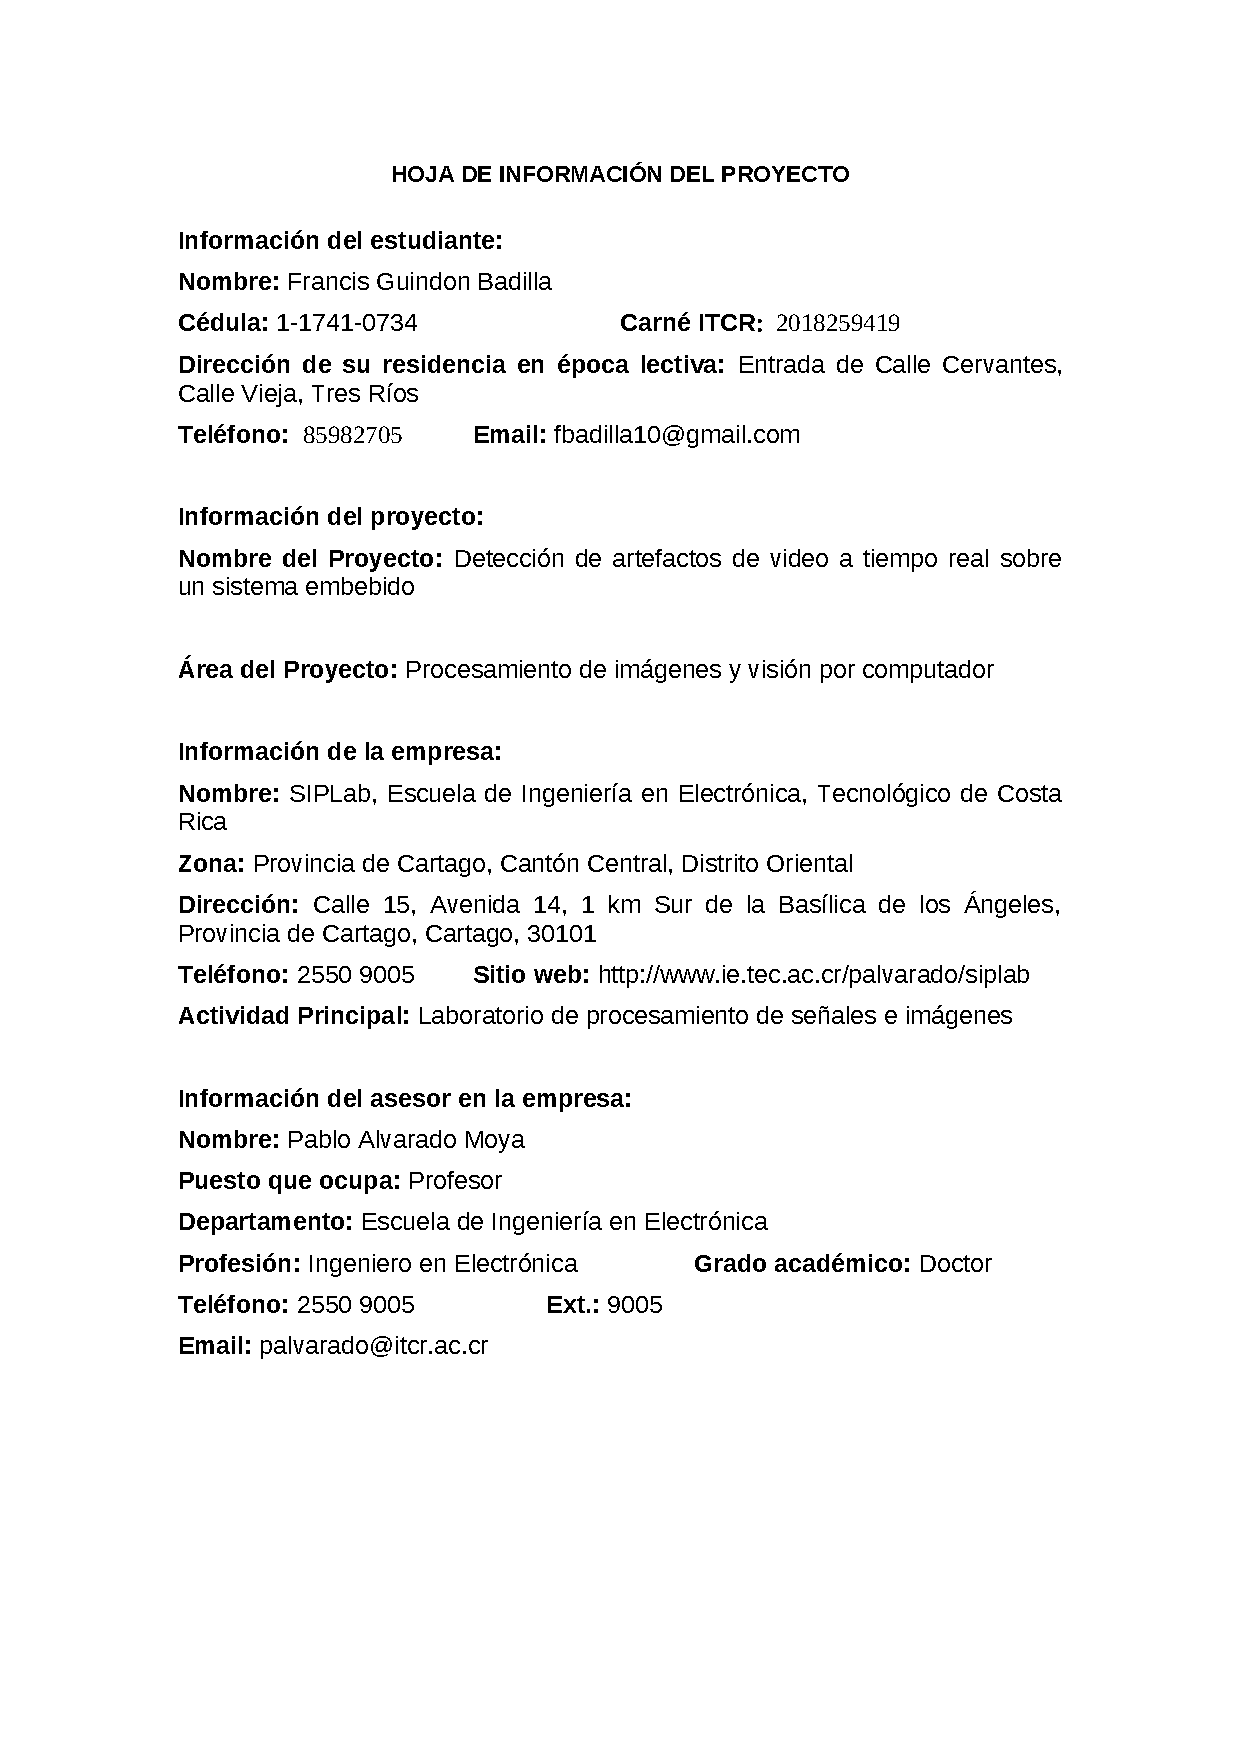
\includepdf[scale=1, offset=3cm -4cm, pagecommand={\textbf{Anexo B}}]{hoja_info.pdf}


  %----------------------------------------------------------------------------
  \backmatter
  %----------------------------------------------------------------------------

  \printindex                % insert index into document. Don't forget to call
                             % "makeindex filename" first.
\end{document}
